%%%%%%%%%%%%%%%%%%%%%%%%%%%%%%%%%%%%%%%%%%%%%%
% To select a journal, use its code for the 
% journal= option in the \documentclass command.
% The journal codes for this template are:
% 
% Annals of Actuarial Science: aas
% British Journal of Political Science: jps
% Network Science: nws
% Political Analysis: pla
% Political Science Research and Methods: ram
% Evolutionary Human Sciences: ehs
% Natural Language Processing: nlp
%%%%%%%%%%%%%%%%%%%%%%%%%%%%%%%%%%%%%%%%%%%%%%
\documentclass[year=2026]{cup-journal}
\usepackage[utf8]{inputenc}

% Force surname-first for ALL authors (APA-like ordering)
\DeclareNameAlias{sortname}{family-given}
\DeclareNameAlias{default}{family-given}

\usepackage{amsmath}
\usepackage[nopatch]{microtype}
\usepackage[hypcap=false]{caption}
\usepackage{booktabs}
\usepackage{caption}
\usepackage{newunicodechar}
\newunicodechar{₃}{$_3$}
\setlength\bibitemsep{0.5em}

\usepackage{xcolor}
\definecolor{linknavy}{RGB}{0,51,102}
\usepackage{hyperref}
\hypersetup{
    colorlinks=true,
    linkcolor=black,
    citecolor=black,
    urlcolor=linknavy,
}

\makeatletter
\renewcommand{\@maketitle}{%
  \setlength\parindent{\z@}%
  \newpage\vspace*{\dimexpr-\headsep-\headheight\relax}%
  % journal line, year/volume/pages, ARTICLE label, and CUP logo all removed
  \vspace*{\cup@space@pre@title}%
  {%
    \titlefont
    \titlesize
    \let\@fnsymbol\cup@author@fnsymbol
    \let\footnote@org\footnote
    \let\footnote\cup@title@footnote
    \cup@maketitle@suppinfo \@title
    \cup@title@footnote@check
    \global\cup@footnote@cnt\c@footnote
    \@maketitle@title@hook
    \par
  }%
  \vspace*{\cup@space@post@title}%
  {\authorsize\authorfont\frenchspacing \cup@author@list \par}%
  \vspace*{\cup@space@post@author}%
  {\affilsize\affilfont \cup@address@list \par}%
  \vspace*{\cup@space@post@address}%
  {%
    \emailsize\emailfont
    \ifcup@email
      \expandafter\cup@contact@details
      \par
      \vspace*{\cup@space@post@email}%
    \fi
  }%
  {%
    \datesize\datefont
    \ifcup@dates
      (Received \cup@recvd; revised \cup@revd; accepted \cup@accptd)%
      \vspace*{\cup@space@post@date}%
    \fi
    \ifcup@copyright
      \bgroup\let\thefootnote\relax
      \footnote{\cup@copyright@notice}%
      \egroup
    \fi
  }%
}
\renewcommand{\ps@plain}{%
  \renewcommand{\@oddhead}{\hfill\thepage}%
  \renewcommand{\@evenhead}{\thepage\hfill}%
  \renewcommand{\@oddfoot}{}%
  \renewcommand{\@evenfoot}{}%
}
\makeatother
\pagestyle{plain}

\title[OpenCitations coverage at UniBO]{In the World of Citations, Are We Really Open(Minded), or Stuck in a Comfort Zone? \\[0.4em]
\normalsize An OpenCitations-based Investigation of Citation Patterns Across Countries and Disciplines in Six Italian Institutions}
\received{June 2026}

\author{Yiğit Ak}
\author{Tommaso Barbato}
\author{Qinghao Chen}
\author{Nicol D'Amelio}
\author{Maryam Dadrasrazi}
\author{Ilaria De Dominicis}
\author{Yi Hua Li}
\author{Regina W.K. Manyara}
\author{Shiho Nakamura}
\author{Miriana Pinto}
\author{Sara Roggiani}
\author{Tianchi Yang}
\author{Peize Yu}
\affiliation{University of Bologna, Bologna, Italy}

\addbibresource{bloom_references.bib}

\keywords{Bibliographic metadata, Citation analysis, Citation data, Disciplinary flows, Geographic bias, IRIS, Italian universities, OpenCitations, Open Data pipeline, Open Science}

\begin{document}

\begin{abstract}
The study analyzes the geographic and disciplinary citation networks of six Italian universities (UNIBO, UNIMI, UNITO, UNIPD, UPO, and SNS) using data from OpenCitations, an open scholarly infrastructure. It evaluates whether these institutions possess distinct research profiles and determines if their citation flows reflect global engagement or are constrained by institutional, geographic, and disciplinary biases.

Utilizing a reproducible, open-data pipeline, publication records were enriched via persistent identifiers. To map geographic flows, records were matched using the OpenAIRE Graph and the Research Organization Registry (ROR). For disciplinary flows, venue metadata from OpenCitations Meta, SCImago Journal Rank (SJR), and the Directory of Open Access Journals (DOAJ) was integrated and standardized using the top-level Library of Congress Classification (LCC).

Geographic mapping reveals a heavy reliance on Western hubs (Western Europe and Northern America), with a stark citation asymmetry regarding China, which acts as a heavy knowledge consumer of Italian research without reciprocal citation. Disciplinary flows are dominated by Science (32.6\%) and Medicine (30.7\%), which exhibit high self-citation rates. Conversely, mid-range fields like Geography and Social Sciences display high cross-disciplinary activity (~80\%). Large generalist universities (UNIBO, UNIMI) maintain vast global networks, while smaller specialized institutions exhibit distinct structures.

This project validates open scholarly infrastructures as transparent, viable alternatives to proprietary databases for mapping complex scientific interactions. Beyond validating the use of open bibliographic data, the study identifies promising directions for future development. In particular, integrating geographic and disciplinary dimensions could enable more fine-grained analyses of institutional profiles and collaboration patterns, further strengthening the analytical potential of open scholarly infrastructures.

\end{abstract}

\section{Introduction}
Citations represent a fundamental mechanism of scholarly communication, forming the basis through which scientific knowledge is acknowledged, connected, and further developed. Beyond their formal role in academic writing, citations reflect intellectual influence and shape the structure of knowledge production across disciplines and research communities. Because of this central role, citation practices offer an important lens through which to study how knowledge circulates within and across academic fields.

Citation practices are often influenced by disciplinary, institutional, and geographical contexts, which can shape patterns of knowledge selection and visibility in scientific communication. In practice, this means that the references included in scientific work are not only the result of individual scholarly choice, but also reflect broader structures within academia, such as established research communities, dominant disciplinary traditions, and regional or institutional proximity. As a consequence, citation patterns can provide insight into how knowledge is distributed and connected across different fields and countries, highlighting the underlying organization of scientific communication. Studying these patterns therefore allows for a better understanding of how research visibility is structured and how certain areas of knowledge become more central than others within the global scientific system.

Previous research in bibliometrics and scientometrics has extensively studied citation behavior as a way to understand how scientific knowledge is produced and disseminated. Citation networks have been shown to exhibit strong structural properties, including inequality in citation distribution and the tendency for highly visible work to attract disproportionate attention, a phenomenon often described as “cumulative advantage” or the “Matthew effect” in science (Merton, 1968). Moreover, network-based approaches have demonstrated that scientific communication is not random, but follows a self-organizing pattern governed by preferential attachment, a “rich-get-richer” phenomenon where highly cited papers naturally attract further citations (Barabási \& Albert, 1999), with disciplinary communities and institutional affiliations playing a central role in shaping these localized citation flows.

More recent studies have further highlighted the existence of geographical and linguistic patterns in citation practices, suggesting that researchers are more likely to cite work produced within similar regional or institutional contexts, with these effects varying significantly across disciplines (Wu et al., 2026). This has led to growing interest in understanding how disciplinary boundaries and national research systems influence the visibility and diffusion of knowledge. At the same time, previous literature such as Leydesdorff \& Persson (2010) and Abramo et al. (2020), has often focused on global or macro-level patterns, while less attention has been given to more fine-grained analyses combining disciplines, institutions, and countries within specific national contexts. This creates a space for further investigation into how citation patterns manifest at the institutional level, particularly within higher education systems such as Italian universities.

In addition to geographical and institutional factors, disciplines represent another fundamental dimension shaping citation behaviour. Despite growing interdisciplinarity and the increasing fluidity of disciplinary boundaries (Brew, 2008), disciplines remain key organisational structures of academic research. Porter and Rafols (2009) found that researchers increasingly draw on knowledge from multiple fields, but that these connections tend to occur primarily between cognitively related disciplines rather than across distant domains. This suggests that disciplinary boundaries have become more permeable without disappearing altogether. Similarly, McLevey et al. (2018) show that citation flows may cross disciplinary boundaries, but academic recognition remains largely discipline-specific. Their findings suggest that citations not only reflect knowledge diffusion but also reinforce disciplinary communities, as scholars tend to assign greater value to recognition received from within their own field. Together, these studies highlight the importance of considering disciplinary structures when analysing citation practices and patterns of scholarly visibility.

However, research evaluation and bibliometric analyses have traditionally relied heavily on commercial databases such as Web of Science and Scopus (Leydesdorff \& Persson, 2010; Abramo et al., 2020; Bol et al., 2023). Nevertheless, the increasing availability of open infrastructures, including \href{https://opencitations.net/}{OpenCitations}\footnote{\url{https://opencitations.net/}}, \href{https://openalex.org/}{OpenAlex}\footnote{\url{https://openalex.org/}}, \href{https://www.openaire.eu/}{OpenAIRE}\footnote{\url{https://www.openaire.eu/}}, \href{https://www.crossref.org/}{Crossref}\footnote{\url{https://www.crossref.org/}}, \href{https://datacite.org/}{DataCite}\footnote{\url{https://datacite.org/}}, and others, has opened new possibilities for conducting analyses based on openly available research information.

The study of citation structural patterns lies at the very heart of the Measurement School, one of the five conceptual pillars defining the modern Open Science movement (Fecher \& Friesike, 2014). This school of thought focuses on developing alternative standards to evaluate scientific impact, arguing that traditional metrics have long held a restrictive stranglehold over research evaluation, funding, and career progression. By treating citations as open digital traces embedded directly within the scholarly workflow, the Measurement School advocates for faster, more transparent evaluation frameworks that accurately capture the diverse ways research is utilized, debated, and disseminated in a digital ecosystem.

More broadly, Open Science serves as an umbrella term for a diverse array of practices designed to open the entire research lifecycle, from initial knowledge creation to its ultimate public dissemination. Beyond this measurement-centric focus, the movement is driven by four other distinct pillars - the Infrastructure, Public, Democratic, and Pragmatic schools - which collectively foster an ecosystem defined by shared technological architecture, public engagement, equitable access to knowledge, and collaborative efficiency (Fecher \& Friesike, 2014). Together, these pillars promote a vision where research outputs, including datasets and code, are governed by the FAIR Guiding Principles proposed by the \href{https://force11.org/}{FORCE11}\footnote{\url{https://force11.org/}} community. By ensuring that data remains Findable, Accessible, Interoperable, and Reusable, this framework shifts research culture away from traditional barriers toward a globally inclusive ecosystem where scientific discovery is accelerated, fully reproducible, and treated as a public good (Wilkinson et al, 2016).

In recent years, the Open Science movement has increasingly promoted such transparency, accessibility, and reproducibility throughout the research lifecycle. Within this framework, international initiatives such as the \href{https://sfdora.org/read/}{San Francisco Declaration on Research Assessment} (DORA)\footnote{\url{https://sfdora.org/read/}}, the \href{https://coara.eu/agreement/the-agreement-full-text/}{Coalition for Advancing Research Assessment} (CoARA)\footnote{\url{https://coara.eu/agreement/the-agreement-full-text/}}, and the \href{https://barcelona-declaration.org/}{Barcelona Declaration on Open Research Information}\footnote{\url{https://barcelona-declaration.org/}} have further highlighted the importance of reducing dependence on proprietary research information systems and fostering the adoption of open scholarly infrastructures.

Among these infrastructures, OpenCitations has gained increasing attention as a provider of openly available citation and bibliographic data. OpenCitations is an open-science initiative established in 2010 which publishes bibliographic citation data in RDF format and maintains the OpenCitations Corpus (Peroni \& Shotton, 2020). It represents a particularly valuable source for citation analysis due to its commitment to data quality and transparency. Citation links included in its indexes undergo validation procedures designed to identify and exclude invalid or malformed identifiers, thereby reducing the presence of erroneous citation relationships (Cioffi et al., 2022).

Interestingly, a more recent study by Andreose et al. (2026) demonstrated that OpenCitations provides substantial coverage of publications and citations included in the IRIS Current Research Information Systems (CRIS), a software adopted by several Italian universities that facilitates the collection, management, and monitoring of information related to research activities and outputs, providing researchers, administrators, and evaluators with tools to document research results and enhance their visibility (Bollini et al., 2016). Andreose et al.’s  analysis showed a promising level of publication and citation coverage and suggested that open infrastructures may already represent a viable alternative to proprietary citation databases in several research assessment scenarios. The results of their work constitute an important step in evaluating the completeness and reliability of OpenCitations data. 

As previously stated, citations are not merely indicators of scholarly impact. They also represent connections among researchers, institutions, countries, and disciplinary communities, making it possible to reconstruct the structure of scientific communication and the circulation of knowledge. While previous studies - like Andreose et al.’s (2026) - focused on assessing the coverage and completeness of open research information sources, less attention has been devoted to exploring the citation relationships that can be reconstructed through such infrastructures. Therefore, this study moves from a quantitative assessment of data availability to an investigation of the citation relationships encoded in such data. The aim of this work is to investigate whether open citation data can be used not only as a source for research assessment but also as a means to reconstruct institutional, geographical and disciplinary citation patterns within the Italian scholarly system.

Moreover, the aforementioned principles of open science promote openness, inclusivity, and the broad dissemination of knowledge (Fecher \& Friesike, 2014), but an important question remains: how open are researchers in their citation practices? When selecting sources, do scholars engage with research from a wide range of disciplines, institutions, and countries, or do they tend to remain within familiar academic networks and disciplinary boundaries? Citation patterns may reveal the existence of “comfort zones” in scholarly communication, where researchers repeatedly cite work from the same countries, institutions, or fields. Such tendencies can limit exposure to alternative perspectives and reduce opportunities for interdisciplinary exchange. Consequently, researchers may unknowingly be reinventing the wheel, reproducing ideas and solutions that have already been explored elsewhere rather than building upon insights developed in other disciplines or regions. By examining citation patterns across disciplines, institutions, and countries, this study seeks to investigate whether scholarly communication truly reflects the ideals of openness and diversity promoted by open science, or whether underlying geographic, institutional, and disciplinary biases continue to shape the production and circulation of knowledge.

In order to investigate the matter, our study focuses on the following research questions:

\begin{enumerate}   
    \item What are:
    \begin{enumerate}
        \item the institutions and countries that either cite or are cited by the IRIS publications included in OpenCitations of a given institution?
        \item the scholarly disciplines that either cite or are cited by the IRIS publications included in OpenCitations of a given institution?
    \end{enumerate}
    \item Are different institutions showing different citation patterns, depending on the specific case (1.a or 1.b)?
\end{enumerate}

To answer these questions, we extend the methodological framework of Andreose et al. (2026) by analysing incoming and outgoing citation flows at the institutional level and integrating disciplinary and geographical metadata within an open-source Python workflow designed to ensure reproducibility.

The study relies on citation data available through OpenCitations and on publication records extracted from the IRIS systems of participating Italian universities. Incoming and outgoing citation relationships were identified and quantified, and the resulting records were enriched with metadata obtained through external APIs. The Italian universities taken into consideration for the analysis are the same for which Andreose et al. (2026) collected data and produced the \verb|iris_oc_mapper|, hence: the University of Bologna (UNIBO), the University of Milan (UNIMI), the University of Padua (UNIPD), the University of Turin (UNITO), the University of Eastern Piedmont (UPO), and the Scuola Normale Superiore (SNS). To advance the vision of a decentralized meta-infrastructure proposed by the same aforementioned researchers, the current project integrates data from OpenCitations and OpenAIRE to support a shared network of open research information. This approach aligns with the previous study’s recommendation to foster a federation of interoperable providers, which they identify as a crucial strategy for bridging coverage gaps, particularly in the Social Sciences and Humanities, and establishing a transparent alternative to proprietary databases as mandated by the Barcelona Declaration (Kramer et al., 2024).

The remainder of this article is organised as follows. Section 2 describes the data sources and methodology adopted for the analysis. Section 3 presents the results obtained for each research question. Section 4 discusses the findings in relation to previous studies and the broader context of open research information, along with its limitations. Finally, Section 5 concludes the article and outlines possible directions for future.

\section{Materials and Methods}

In order to address the project's research objectives, the research team was divided into two working groups, each responsible for a separate research question and methodological workflow. While both investigations relied on institutional bibliographic data, they focused on different analytical perspectives and therefore required distinct data processing procedures.

To ensure transparency and reproducibility, all source code, documentation, and supporting materials are openly available in the project repository hosted on \href{https://github.com/open-sci/2025-2026}{Github}\footnote{\url{https://github.com/open-sci/2025-2026}}. Detailed and reproducible descriptions of the workflows are provided through dedicated protocols: one for \href{https://dx.doi.org/10.17504/protocols.io.yxmvm86kbg3p/v3}{Research Question 1A (RQ 1A)}\footnote{\url{https://dx.doi.org/10.17504/protocols.io.yxmvm86kbg3p/v3}} and one for Research Question 1B (RQ 1B) (https://dx.doi.org/10.17504/protocols.io.dm6gp7nw1gzp). Additional information regarding data management, storage, preservation, and sharing is available in the project's \href{https://zenodo.org/records/20159031}{Data Management Plan (DMP)}\footnote{\url{https://zenodo.org/records/20159031}} published on Zenodo.

\subsection{Source Data}

As previously stated, this project expands the work done by Andreose et al. (2026) who performed an analysis looking at the coverage of Italian publications in OpenCitations. The resulting dataset  from their analysis was constructed by matching publications recorded in the six IRIS installations against OpenCitations Meta using persistent identifiers (DOIs, PMIDs, and ISBNs), and extracting the corresponding citation links from the OpenCitations Index. This dataset acted as the basis for our own investigation. 

The dataset, publicly available on \href{https://doi.org/10.5281/zenodo.18202530}{Zenodo}\footnote{\url{https://doi.org/10.5281/zenodo.18202530}}, is organised into one folder per institution, each containing two key files, \verb|iris_in_oc_meta|, which provides basic bibliographic metadata for IRIS publications recognised in OpenCitations Meta; \verb|iris_in_oc_index|, which contains all citation relationships extracted from OpenCitations Index involving any of those publications. 

In the context of our investigation, both research questions are interested in exploring the features (cross-institution, cross-country, cross-discipline) of each institution's research outputs, therefore we first leveraged the \verb|iris_in_oc_index|. Each record in this file represents a citation pair and includes the following fields: a unique OC Index citation identifier (\verb|id|), the OMID of the citing publication (\verb|citing|), the OMID of the cited publication (\verb|cited|), the creation date of the citation (\verb|creation|), and two boolean flags (\verb|is_citing_iris|, \verb|is_cited_iris|) indicating whether the citation is coming from or going towards the relevant IRIS institution. The \verb|iris_in_oc_meta| was only used for the country-level analysis, serving to resolve OMIDs into persistent identifiers such as DOIs and PMIDs, which were required to retrieve the author affiliations and geographic data necessary.

\subsection{Map of Italian Science Methodology}

The following workflow describes the methodological framework for mapping the international reach of Italian academic research (RQ 1A). This process transforms raw institutional citation data into a comprehensive geographic and organizational dataset, enabling the analysis of citation flows across global borders and research entities.

The first phase, \textit{Initial Dataset Preparation and PID Enrichment}, focuses on reconstructing the bibliographic context of institutional research by enriching raw citation indices with persistent identifiers (PIDs). Using institutional IRIS citation datasets as a starting point, which list citation pairs involving publications already recognized in OpenCitations, the workflow streams the OpenCitations Meta database. This streaming process allows for the resolution of internal OpenCitations Meta Identifiers (OMIDs) into standardized PIDs, such as DOIs, PMIDs, and ISBNs, along with publication dates. During this stage, citation directions are explicitly defined as incoming, outgoing, or internal based on the IRIS membership flags of the citing and cited publications, creating a foundational enriched index for subsequent mapping.

To ensure accurate mapping at the country and institution level, the second phase establishes a normalized lookup for research organizations. This is achieved by combining the \href{https://graph.openaire.eu/docs/}{OpenAIRE Graph}\footnote{\url{https://graph.openaire.eu/docs/}} organization records with the \href{https://ror.readme.io/docs/rest-api}{Research Organization Registry (ROR)}\footnote{\url{https://ror.readme.io/docs/rest-api}}. By indexing ROR identifiers to display names and geographic location data, the workflow creates a robust mapping that prioritizes ROR-validated country codes and names, falling back to OpenAIRE’s internal geographic metadata only when necessary. This ensures that affiliations are assigned to a stable geographic and institutional hierarchy.

The third phase represents the most computationally intensive stage, where publications are linked to their authors' institutional affiliations. By scanning the OpenAIRE publication and relation dumps, the workflow matches the enriched PIDs from Phase 1 to specific OpenAIRE publication IDs. It then extracts author-affiliation relations to identify the organizations associated with each research output. These organizations are then resolved through the ROR-enriched lookup developed in the previous phase, resulting in a finalized mapping of publications to specific countries and research entities.

Once the bibliographic and organizational data are aligned, the workflow moves to data aggregation. For each of the six universities considered, the system systematically counts the organizations and countries involved in its citation network. For incoming citations, the citing publication's organizations are recorded as external sources; for outgoing citations, the cited publication's organizations are recorded as targets. To ensure accuracy, organization lists are deduplicated at the publication level, preferring ROR identifiers to consolidate counts across varied naming conventions. This phase culminates in the production of per-university citation-count tables aggregated by both organization and country. In the production of the counts, the Integer Counting method is adopted, assigning a weight of 1 (full citation action) to every organization or country identified within a citation pair. This choice is driven not only by a commitment to transparency and reproducibility - avoiding the “fractional artifacts” that can complicate the interpretation of results - but also by the specific nature of the OpenAIRE metadata used in this study. Given that OpenAIRE data can occasionally be fragmented and that many publications involve a very high number of affiliated institutions, applying a fractional counting approach would risk systematically underrepresenting many actors by diluting their contribution into negligible, infinitesimal values. Conversely, Integer Counting ensures that every institutional and geographic connection is clearly surfaced, preserving the integrity of knowledge flows even within large-scale international collaborations.

To maintain the principles of Open Science, every stage of the pipeline produces explicit intermediate files and metadata summaries, ensuring that records that cannot be resolved are documented rather than discarded. To facilitate full reproducibility, all scripts, protocols, and resulting datasets are made publicly available also in the \href{https://github.com/open-sci/2025-2026/tree/main}{project GitHub repository}, which has been previously mentioned.

\subsection{Disciplinary Flow Methodology}

The workflow developed for RQ 1B consists of three sequential phases designed to transform raw citation relationships associated with institutional publications into a harmonised disciplinary dataset suitable for analysing citation flows across fields of research.

The first phase, \textit{Data Gathering and Metadata Enrichment}, aimed to reconstruct the disciplinary context of the publications involved in the citation network. Since citation records alone do not provide explicit information about the scholarly disciplines associated with the citing and cited publications, additional journal-level metadata had to be collected and integrated. To this end, all citation pairs extracted from the institutional datasets were enriched with venue information retrieved from the OpenCitations Meta database. OpenCitations Meta provides structured bibliographic metadata describing scholarly resources and their publication venues, including identifiers such as ISSNs, which can be used to connect publications to external classification systems. After extracting ISSNs from the retrieved venue metadata, journals were matched against two complementary disciplinary classification sources: the \href{https://doaj.org/}{Directory of Open Access Journals (DOAJ)}\footnote{\url{https://doaj.org/}}, which assigns subject categories based on the \href{https://www.loc.gov/catdir/cpso/lcco/}{Library of Congress Classification (LCC) scheme}\footnote{\url{https://www.loc.gov/catdir/cpso/lcco/}}, and \href{https://www.scimagojr.com/}{SCImago Journal Rank (SJR)}\footnote{\url{https://www.scimagojr.com/}}, which provides journal classifications derived from the Scopus taxonomy. The result of this phase was a citation dataset in which both the citing and cited publications were associated, whenever possible, with one or more disciplinary labels.

The second phase, \textit{Disciplinary Alignment and Standardisation}, addressed the heterogeneity of the classification systems used by the two sources. Because DOAJ and SJR adopt different taxonomies and levels of granularity, a common disciplinary framework was required to enable meaningful comparisons across institutions and data sources. For this reason, all disciplinary labels were mapped to the top-level classes of the Library of Congress Classification (LCC), which was adopted as the reference taxonomy for the analysis. The LCC was selected because it is a well-established and widely used knowledge organisation system that provides broad disciplinary coverage across the sciences, social sciences, humanities, and applied fields. Its hierarchical structure also facilitates the aggregation of heterogeneous classification schemes into a shared framework without favouring the disciplinary logic of a specific database. Restricting the classification to the highest level of the hierarchy (21 classes in total) ensured a balance between disciplinary specificity and interpretability, while reducing fragmentation caused by highly specialised categories and minimising inconsistencies arising from differences in source-level classifications. At the end of this phase, each citation record contained standardised disciplinary assignments for both the citing and cited entities.

The third phase, \textit{Data Aggregation}, transformed publication-level citation records into discipline-level citation relationships. Citation pairs were aggregated into disciplinary edge lists representing flows between source and target disciplines. Whenever journals were associated with multiple disciplinary labels, all valid discipline-to-discipline combinations were generated through Cartesian expansion to preserve the multidisciplinarity of the original records. Each resulting edge retained information about the citation direction and institutional context, allowing us to distinguish among incoming, outgoing, and internal citation flows. This phase produced a structured representation of disciplinary interactions suitable for quantitative analysis.

Throughout the workflow, records that could not be processed due to missing or incomplete information, for example unavailable venue metadata, missing ISSNs, or unsuccessful classification matches, were not discarded. Instead, they were stored separately at each stage of the pipeline in dedicated CSV files. This approach ensured transparency in the processing workflow, facilitated error tracking and quality assessment, and allowed us to quantify the impact of missing information on the final disciplinary coverage. Figure 2 provides a Sankey diagram of the data processing workflow, illustrating the proportion of data retained and lost at each stage of the filtering and processing pipeline.

\section{Results}

\subsection{Map of Italian Science Results (RQ 1A)}
The methodologies presented in the previous section produced the following results, which address the research questions outlined in the introduction. For the country-level analyses, Italy is included in Table 1 in order to provide a complete overview of the citation relationships involving the selected institutions. As for the visualization of these analyses, Italy is excluded from the country-level visualizations because it consistently appears among the top citation partners of all six evaluated institutions and invariably ranks within the top three. Its inclusion would therefore dominate the visual representations and obscure patterns involving foreign countries. On the other hand, for the institution-level visualizations included in the paper, Italy is retained because relationships among Italian institutions are important and highly relevant to future research directions. Interactive visualizations on the \href{https://open-sci.github.io/2025-2026/}{project website}\footnote{\url{https://open-sci.github.io/2025-2026/}} allow for further exploration of institution-level relationships with Italy excluded.

In the context of this study, “partner countries” refer to all countries that are either cited by or cite the selected institutions. Accordingly, citing countries correspond to incoming citation flows, while cited countries correspond to outgoing citation flows.

At a macro level, the geographic distribution of citation flows reveals a highly isomorphic pattern across all six Italian institutions, demonstrating that this academic framework shares a common citation skeleton. To accurately map both volume and relationship dynamics across these networks, analytical adjustments such as logarithmic scaling, which visually compresses extreme disparities in raw citation counts, and asymmetry ratios, a log-base-2 metric evaluating the directional balance of outbound to inbound citations, were utilized.

Table 1 outlines the top 20 citing and cited countries, highlighting the foundational architecture of Italy’s international scientific exchange. Many of the evaluated institutions are consistently connected to the same core countries. The United States, France, the United Kingdom, and Germany consistently emerge as dominant hubs. However, analyzing the directional balance uncovers distinct structural asymmetries. The United States is the most important citation partner in terms of absolute volume but shows a strong outgoing skew, indicating Italian researchers cite American publications at a vastly higher rate than they are cited in return. Conversely, relationships with European peers demonstrate a significantly more balanced equilibrium, with countries like France displaying a remarkably symmetric, bilateral exchange. A notable anomaly is the relationship with China, which shows a stronger incoming skew; Chinese academics cite Italian research heavily, but Italian researchers cite China at a substantially lower relative rate.

While the data suggests a shared international structure, isolating relative geographic specialization reveals distinct institutional fingerprints. The larger, multidisciplinary research universities boast massive citation traffic and a widely distributed global footprint. However, differences emerge when comparing large and small universities. For example, countries such as Turkey, Russia, and India sometimes fluctuate in institutional rankings, a variance that is especially pronounced for the smaller universities. Smaller institutions often display more diverse citation profiles relative to their scale; because they produce fewer publications, their citation networks are less concentrated in a limited set of high-volume international relationships.

To further unpack this institutional variance, Figure 3 and Figure 4 utilize heatmaps to explain how individual institutions deviate from national-level citation patterns. By mathematically subtracting the overwhelming macro-level dominance of the core countries, these visualizations reveal which relationships are stronger or weaker than expected. Consequently, the heatmaps expose unique geographic specializations and relative institutional footprints that cannot be seen from simple volume rankings.

The results reveal that most institutions closely follow a common international citation structure, with only modest deviations from the group average. However, SNS and UPO emerge as the most distinctive cases. SNS exhibits a stronger orientation toward the United States and Russia, alongside a comparatively weaker connection to China, while UPO shows a more pronounced orientation toward Asian countries such as India, South Korea, and China and a lower-than-average reliance on the United States. UNIMI displays the strongest relative emphasis on citations involving the United Kingdom and the United States, whereas UNIPD shows the most pronounced French orientation in both incoming and outgoing citation flows. In contrast, countries such as Brazil and Switzerland exhibit near-uniform patterns across all institutions, suggesting broadly shared citation relationships. These findings indicate that although Italian universities operate within a common global citation framework, institutional citation profiles still reflect distinct disciplinary compositions and strategic orientations.

Further structural dynamics are illustrated in Figure 5 and Figure 6, which visually map international dependencies through citation asymmetry. The two figures showcase examples of one big university, UNIBO, and one smaller one, SNS. These visualizations plot the relative directional exchange rate calculated as a base-2 logarithm of the ratio of outbound to inbound citations. Under this logarithmic framework, a value of zero indicates perfect structural balance, signaling a symmetric, reciprocal academic exchange. Positive values denote an outgoing citation bias, where the institution predominantly acts as a consumer of that nation’s scientific literature, while negative values indicate an incoming citation bias, where the institution acts as a net exporter of knowledge. At first glance, Italy appears highly dependent on the United States due to the sheer volume of citations exchanged. However, the asymmetry analysis reveals a more nuanced picture. While the United States remains one of the largest citation sources, the relationship is not as unidirectional as raw citation counts alone might suggest. More broadly, the asymmetry maps show that the majority of countries fall on the incoming side of the scale, indicating that Italian institutions generally receive more citations than they produce toward those countries. This pattern is particularly evident for four of the six universities examined (specifically UNIBO, UNIMI, UNITO and UNIPD), where incoming citation flows systematically exceed outgoing ones. China, despite its large citation volume, also exhibits a noticeable incoming imbalance rather than a perfectly reciprocal exchange. Overall, the results suggest that these Italian institutions function more as receivers of international scientific attention than as consumers of foreign literature, although the magnitude of this effect varies across countries and institutions.

The strongest asymmetries are often observed among smaller and emerging scientific systems, including several countries in the Global South, where citation exchanges tend to be particularly uneven. By comparison, relationships with major research-producing countries such as the United States and leading European partners generally exhibit more balanced citation exchanges, even when substantial asymmetries remain present.

Furthermore, a major structural finding emerges when analyzing SNS (Fig. 6), which presents a distinct citation profile that breaks the patterns observed in the larger universities. In sharp contrast to the other five universities, where the United States consistently exhibits a pronounced outgoing consumer bias, the relationship between SNS and the United States is almost perfectly balanced.

To reduce statistical noise from very small citation relationships, only countries with a threshold of at least 500 citations were included in this specific asymmetry mapping.

Transitioning from country-level to organizational-level analysis allows for an examination of whether international citation relationships are concentrated in a few prestigious institutions or broadly distributed. Figure 7 maps these inter-institutional flows through a diverging bar chart, while Table 2 details specific relational ratios. Analyses of citation volume versus concentration, alongside the Concentration Ratio at N = 3 (CR₃), which measures the contribution of the top three organizations to a country’s total citation volume, reveal a clear structural pattern: countries with the largest citation volumes consistently exhibit the lowest concentration levels, indicating that their citation relationships are distributed across a broad range of organizations. In contrast, countries with smaller citation volumes tend to display substantially higher CR₃ values, meaning that their interactions are often driven by one or two dominant institutions. This suggests that large citation networks correspond to mature and system-wide forms of engagement, whereas smaller networks frequently reflect more localized or bilateral partnerships. The near-zero CR₃ values observed for major partner countries therefore indicate genuinely broad participation across dozens of entities rather than fragile hub-and-spoke structures. Additionally, some organizations function primarily as publishers, such as Harvard University Press, and consequently exhibit distinct concentration patterns as dominant outgoing sinks. Overall the two organizations that stand out across the dataset are Centre national de la recherche scientifique (CNRS) from France and Harvard University Press from the United States.

Reciprocity findings generated from the scatter analysis, provided in the \href{https://github.com/open-sci/2025-2026/blob/main/bloom/map_of_italian_science/data_viz/organization_level_analysis.ipynb}{jupyter notebook}\footnote{\url{https://github.com/open-sci/2025-2026/blob/main/bloom/map_of_italian_science/data_viz/organization_level_analysis.ipynb}} and on the \href{https://open-sci.github.io/2025-2026/}{project website}, map the dynamic between incoming and outgoing citations at the organizational level. A key structural feature is that incoming diversity exceeds outgoing diversity at every institution; Italian universities are cited by a broader range of partner organizations than they actively cite. Furthermore, each institution maintains a distinct citation balance. UNIMI attracts the most incoming citations relative to outgoing, while UNITO has the most outgoing citations compared to incoming, acting as the strongest net citation importer. In contrast, SNS achieves the most symmetric exchange overall and is uniquely characterized by its ties with CERN as a dominant partner, rather than traditional publishers. Overall, the scatter plots display a structural symmetry with a distinct directional nuance: outgoing citation counts are systematically lower than incoming counts, indicating that these Italian institutions receive citations from a wide global base while maintaining slightly more selective outgoing reference lists.

Finally, the team proceeded with a temporal analysis, which adds an evolutionary dimension by showing how citation structures change over time. Across the five 5-year periods, included between 2001 and 2025, the dominant trajectory is characterised by simultaneous growth in citation volume and declining concentration. Table 2 reports the CR values exclusively for the endpoints of the observed timeframe, facilitating a clearer interpretation of the rate's evolution. Most partner countries move rightward and downward in the \href{https://github.com/open-sci/2025-2026/blob/main/bloom/map_of_italian_science/data_viz/countries_organizations_analysis.ipynb}{animated scatter plots}\footnote{\url{https://github.com/open-sci/2025-2026/blob/main/bloom/map_of_italian_science/data_viz/countries_organizations_analysis.ipynb}}, indicating that expanding citation relationships tend to become distributed across a broader range of organisations. This pattern is particularly evident for countries such as China and India, which evolved from relatively concentrated, moderate-volume relationships in the early 2000s to large-scale, low-concentration networks by 2021-2025. In contrast, major partners such as the United States, the United Kingdom, Germany, and France exhibit consistently low CR₃ values throughout the entire period, reflecting long-standing engagement across extensive institutional ecosystems. Smaller partner countries often remain comparatively concentrated, suggesting that their citation relationships continue to be driven by a limited number of organisations or specialised bilateral collaborations. Overall, the temporal evidence indicates that as citation networks mature and expand, they tend to become structurally more diversified and system-wide rather than dependent on a small set of dominant institutions.

\subsection{Disciplinary Flow Results (RQ 1B)}

To better understand the disciplinary structure of the citation networks associated with the participating institutions, we visualised both the overall distribution of citation activity across disciplines and the citation flows connecting different disciplinary areas. The following analyses highlight the relative importance of each discipline, the balance between citing and cited activity, and the extent to which knowledge circulates within disciplinary boundaries or across different fields.

From the processed aggregated dataset, we obtained a total of 86,150,074 bibliographic records that either cite or are cited by IRIS publications of the six institutions. Table 3 represents the total citation volume per discipline per institution, combining citing and cited counts, together with each discipline's share within its institution. Across all six institutions combined, the distribution was heavily concentrated in two LOC Main Classification categories. Science accounted for 32.6\% of total citing activity across all institutions, and Medicine for 30.7\%, together exceeding 60\% of the total. The remaining disciplines each have far less shares; Geography/Anthropology, Technology, Agriculture, Social Sciences, and Philosophy/Psychology/Religion each contributed between approximately 2–7\% of total volume. Several classification categories such as Fine Arts, Law, and Bibliographic and Library Science resulted in near-zero counts, accounting for less than 1\%.

Figure 8 shows the discipline-level citation volumes as grouped bar charts, one panel per institution, with citing (blue) and cited (red) counts shown side by side for each discipline. While the dominance of Science and Medicine is universal, the balance between the two and the role of secondary disciplines varied markedly across institutions, which we further analyze in the following sections. We can observe that mid-range disciplines tend to show higher citing (blue) than cited volumes across all institutions, suggesting these fields are more active as citation users than as citation recipients, in contrast to Science and Medicine where the cited bar tended to equal or exceed the citing bar.

To reframe the results with UNIBO as a representative example for a given institution to the related research question, UNIBO closely mirrors the macro distribution, with Science standing as the lead category with 31.1\% share followed by Medicine at 26.4\%. The primary core is followed by Geography, Technology, Agriculture, Social Science, Education, Political Science, and Philosophy which together constitute the next distinct structural layer. The top-left UNIBO panel in Figure 8 shows slight asymmetry between inbound and outbound citation: Science disciplines citing UNIBO account for the largest absolute volume; Medicine’s cited count exceeds its citing count. For most disciplines other than Medicine, citing records consistently outnumber cited records.

We examined the directional flows between disciplines by aggregating all citing-cited pairs for each institution. Figure 9 shows the top 10 citing-cited pairs ranked by volume for each institution; the different colors in the bar indicate the citation type (incoming, outgoing, and internal). Consistent with the findings from the disciplinary distribution in the previous section, the top two pairs at five of the six institutions were within-discipline citation between Science and Medicine, and the next two pairs the combination of them. Beyond these four, the remaining ranked pairs are predominantly composed of a third discipline paired with either Science or Medicine, rather than interaction between two non-dominant fields. 

To further investigate citation flow patterns, we broke down each discipline’s citation activity into within-discipline self-citation (pairs within the same discipline) and cross-disciplinary citation (pairs across different disciplines). Figure 10 illustrates the proportions of within-discipline self-citations (Self) and cross-disciplinary citations (Cross) for each institution. Given the significant variance in citation volumes across disciplines, we categorized them into three tiers: High-range (Science and Medicine), Middle-range (Geography/Anthropology, Technology, Agriculture, Social Sciences, and Philosophy/Psychology/Religion), and Low-range (remaining disciplines). Across all six institutions, the dominant fields of Science and Medicine exhibit the largest self-citation shares, while disciplines with lower volume are predominantly cross-disciplinary. Large disciplines tend to cite and be cited within their own field, whereas smaller disciplines rely more heavily on connections with Science or Medicine.

Taking UNIBO as an example again, the ranking of citation pairs align with the overall trend, with the top positions dominated by Science citing Science and Medicine citing Medicine. While the share of within-discipline self-citation is relatively high for these two dominant fields, Figure 10 reveals that around 80\% of the citation activity in mid-range disciplines, such as Geography, Education, and Social Sciences is cross-disciplinary. For a full visual breakdown of directed citation flows between discipline pairs, interactive Sunburst charts and Sankey diagrams are available in the supplementary \href{https://github.com/open-sci/2025-2026/blob/1b/bloom/disciplinary_flow/visualization/viz_discipline_flow.ipynb}{Jupyter notebook}\footnote{\url{https://github.com/open-sci/2025-2026/blob/1b/bloom/disciplinary_flow/visualization/viz_discipline_flow.ipynb}} and the \href{https://open-sci.github.io/2025-2026/}{website}.

\newpage
\section{Discussion}

\subsection{Interpretation}

The empirical findings from the first research question reveal that global knowledge flows are highly stratified, with specific countries exerting an exponentially greater influence on both incoming and outgoing citation volumes across the six Italian universities. What stands out from these results is a distinct geographic division of labor: the United States and core European nations (primarily France, Germany, and the United Kingdom) act as the primary knowledge providers for the Italian academic system. Conversely, China and nations across the Global South appear predominantly as knowledge consumers within this network, citing the Italian research centers significantly more than they are cited in return - a disparity clearly visualized in the asymmetry maps (Fig. 5 \& Fig. 6). Rather than reflecting a purely meritocratic distribution of scientific merit, this attempt at mapping Italian science exposes deeply entrenched cultural and regional biases within transnational citation networks, likely driven by geographical, institutional, and linguistic barriers.

This observed concentration of scientific capital within the West, coupled with the asymmetric consumer status of emerging economies, aligns with a well-documented “core-periphery” structure in global scientometrics literature (Wu et al., 2026). Within this self-organizing framework, an elite core of advanced nations utilizes global knowledge with exceptional efficiency, creating an extreme geographical concentration where nearly a third of the world’s most highly cited researchers reside in just a few dozen Western institutions (Batty, 2003). Moreover, large-scale bibliometric evaluations reveal that while emerging scientific economies rely heavily on Western frameworks, Western researchers exhibit a systematic tendency to under-cite and undervalue work originating from these regions (Wu et al., 2026), just like shown in our results. Such patterns indicate that citation practices remain deeply embedded in localized contexts that naturally favor culturally familiar and regionally close scholarship. This also appears as the reason why Italy is always among the top three most relevant partner countries for all six of the universities taken into consideration in the present study.

Geographical and institutional barriers compound this core-periphery dynamic. Despite digital connectivity, physical distance continues to constrain knowledge diffusion because advanced research retains a “tacit” component dependent on face-to-face interaction and trust, typically fostered at national or continental levels (Abramo et al., 2020). Concurrently, cultural and linguistic biases act as formidable structural hurdles. The Western Europe and Northern America (WENA) group maintains a systemic monopoly over top-ranked journals and commercial publishing, enforcing strict English-language requirements and prestige-based indexing norms that marginalize non-Western research agendas through a “colonial model” of knowledge extraction (Bol et al., 2023). This institutional bias is reinforced by systemic double standards in peer review, where identical research abstracts are consistently rated higher for quality and relevance when blindly attributed to high-income countries rather than low-income nations (Skopec et al., 2020). Controlled experiments have also demonstrated that both researchers and laypersons systematically rate identical scientific methodologies more favorably if the work is attributed to a Western nation like the United States rather than an emerging power like China (Kowal et al., 2022). These psychological and institutional biases sustain a compounding “Matthew Effect” (Merton, 1968), where eminent nations receive disproportionate credit and funding, further isolating researchers operating outside affluent economic zones.

Regional citation biases distort our collective understanding of global science and actively silence valuable scholarly voices (Mattiazzi \& Vila-Petroff, 2024). Various studies have proposed structural interventions, most notably the establishment of independent regional citation databases to challenge the dominance of Western indexing (Bol et al., 2023) and the adoption of reference list reviewers or anonymized submissions to root out institutional prejudice (Skopec et al., 2020). However, we also should confront the reality that perfect objectivity in science is a myth (Giray, 2026); as Giray (2026) believes, because research is conducted by human beings and shaped by institutional and cultural frameworks, bias is not a sign of failure but a condition that must be honestly understood and managed. Ultimately, objectivity should be treated not as a perfectly achievable state, but as a regulative ideal, a guiding direction that researchers can only approach through transparency, reflexivity, and a constant commitment to open-mindedness, even in terms of citations and references selected.

In relation to the second research question of this study, which examines whether the six different institutions analysed exhibit distinct citation patterns, the geographic distribution of partner countries across UNIMI, UNIBO, UNIPD, UNITO, UPO, and SNS is highly homogeneous. The data - also available on the \href{https://open-sci.github.io/2025-2026/}{website} for further exploration - indicates that the United States, France, Italy, China, Spain, Germany, and Japan consistently serve as partner countries for all six Italian universities. Variations among other partner countries are minimal, potentially reflecting the specific areas of expertise of individual institutions; notably, outlier countries appear primarily in the results of Italian universities with smaller citation volumes - such as UPO with India, and SNS with Russia, South Korea, and Turkey. While these partnerships may be driven by the specialized research domains of each university, the lack of granular data regarding the specific fields of expertise of individual institutions has precluded further investigation into this aspect, which will be addressed comprehensively in the limitations section.

On the other hand, when cross-analyzing the six institutions from a disciplinary perspective, besides the dominance of Science and Medicine existing among all, the results seem to reflect the academic focus and structural characteristics of individual institutions. 

The first is the specialized scientific profile of SNS. Compared to the comprehensive universities, SNS shows exceptionally concentrated distribution. Approximately 50\% of its total citation activity is focused within Science, whereas Medicine, which captures a dominant share at other institutions, remains remarkably low at around 11\%. This unbalanced weight on Science establishes SNS as a unique outlier distinct from the other five institutions.

Secondly, there is a distinction among the five remaining institutions in the proportion of Medicine and Science and the rest of the disciplines. UNIMI and UPO particularly has a high concentration in these two areas, with their combined shares reaching 72\% and 75\% respectively, characterising them as a medical and science dominant group. Conversely, UNIBO, UNIPD, and UNITO represent a relatively more balanced distribution. Notably, UNIBO displays the lowest combined share of Science and Medicine among all six institutions, demonstrating a more diverse disciplinary foundation. Within these balanced institutions, UNIPD possesses higher citation counts in Philosophy, Psychology, and Religion, while UNIBO has clusters of social disciplines, including Social Sciences, Education, and Political Science.

Thirdly, regarding cross-disciplinary citation trends, the overall proportion remains relatively uniform at the institutional level, ranging between around 50\% and 60\% across all six universities, as can be seen in Figure 10. However, at a higher granular level, the figures reveal that these rates are related to each institution's specific disciplinary profile. At SNS, as well as the medical/science heavy UNIMI and UPO, the massive volume of these dominant fields drives up within-discipline self-citations. In contrast, the comparatively balanced universities (UNIBO, UNITO, and UNIPD) show a marginally higher cross-disciplinary rate than their peers. 

The results highlight the central role of Science and Medicine across all six institutions, both in terms of citation volume and disciplinary prominence. However, this predominance should be interpreted with caution. As Franssen and Wouters (2019) argue, bibliometric indicators and citation databases have historically been developed around the communication practices of the natural sciences, where journal articles, rapid citation cycles, and international publication channels occupy a central role. In contrast, Humanities disciplines often rely more heavily on books, edited volumes, local languages, and longer temporal horizons of knowledge production and use. Consequently, differences in citation volume and visibility may reflect not only differences in research activity, but also differences in disciplinary communication cultures and in the extent to which these practices are captured by bibliometric infrastructures. The comparatively limited presence of Humanities disciplines in the networks analysed here should therefore not be interpreted as evidence of lower scholarly relevance or influence.

A further methodological consideration concerns the disciplinary classification system itself, as they are not neutral representations of research domains. As shown by Sīle et al. (2021), classification systems reflect the intellectual, institutional, and historical contexts in which they are developed, and the same publication may be assigned to different disciplines depending on the classification adopted. While broad disciplinary patterns are often robust across systems, disciplinary boundaries remain partly constructed rather than objectively given. The distributions observed in this study should therefore be understood as representations of research activity through the lens of a specific classification framework. Moreover, scholarly communication is not determined only by disciplines. It is also shaped by national research systems, evaluation policies, and publication cultures. Even within the same discipline, researchers may publish differently depending on the country in which they work (Petr et al., 2021).

At the same time, the results reveal substantial levels of cross-disciplinary citation across all institutions, with approximately half of the citation flows occurring between different disciplinary areas. These findings are consistent with previous bibliometric studies documenting increasing interdisciplinarity in scholarly communication (Porter \& Rafols, 2009). However, interdisciplinarity should not be interpreted as the disappearance of disciplinary structures. Porter and Rafols observed that most interdisciplinary exchanges occur between cognitively related fields, suggesting that disciplinary boundaries have become more permeable rather than irrelevant. In this sense, the citation networks analysed here point to a scholarly landscape characterised by both disciplinary specialisation and cross-disciplinary interaction.

This interpretation is further supported by broader theoretical perspectives on the nature of disciplines. Hérubel (2021) describes disciplines as fluid configurations of knowledge connected through continuous flows of information and ideas, while Brew (2008) argues that disciplinary identities are increasingly dynamic and interconnected rather than fixed and self-contained. From this perspective, citation flows can be understood not only as indicators of influence but also as traces of knowledge circulation across disciplinary communities. The relatively high proportion of cross-disciplinary citations observed across all institutions suggests that contemporary research increasingly develops through interactions among neighbouring fields and through the integration of diverse perspectives.

Nevertheless, disciplinary structures remain highly influential. The strong concentration of citation activity within Science at SNS, as well as the dominance of Science and Medicine at UNIMI and UPO, demonstrates that institutional research profiles continue to be shaped by disciplinary specialisation. Moreover, as McLevey et al. (2018) argue, citations perform a dual function: they facilitate the diffusion of knowledge across disciplinary boundaries while simultaneously acting as mechanisms of disciplinary recognition and validation. Ideas may travel between fields, yet scholarly prestige and visibility often remain anchored within disciplinary communities. This may help explain why substantial cross-disciplinary citation flows coexist with persistent disciplinary concentrations.

Taken together, these findings suggest that contemporary scholarship cannot be adequately described either as a collection of isolated disciplinary silos or as a fully integrated and boundaryless system. Rather, research appears to operate through partially connected disciplinary communities in which knowledge circulates across fields while institutional structures, evaluation systems, and academic identities continue to be organised around disciplinary categories. Understanding this tension between disciplinary persistence and disciplinary fluidity is essential for interpreting citation patterns and for evaluating the opportunities and limitations of bibliometric approaches to the study of scholarly communication.

\subsection{Limitations}

The results presented in this study should be interpreted in light of several methodological and data-related limitations. First, the disciplinary analysis relies on journal-level classifications derived from DOAJ and SCImago. Consequently, disciplinary assignments reflect the primary subject areas associated with publication venues rather than the specific content of individual articles. This approach is common in bibliometric research but may not fully capture the multidisciplinarity of individual publications. Furthermore, the disciplinary classifications used in this study correspond to the versions of DOAJ and SCImago available at the time of data collection. As journal classifications evolve over time, the disciplinary labels assigned to publications may not fully reflect the classifications that were in use when the cited articles were originally published.

In addition, disciplinary information from different sources was harmonised through the top-level categories of the Library of Congress Classification system. While this standardisation enabled comparisons across datasets, it inevitably reduced disciplinary granularity. Broad categories such as Science and Medicine encompass a large number of heterogeneous subfields that remain indistinguishable in the final analysis. As a result, some citation patterns observed within these domains may reflect the aggregation of diverse disciplinary communities rather than genuine within-discipline interactions.

The study is also affected by data loss occurring throughout the enrichment process. Citation records lacking venue metadata, ISSNs, or valid matches in the disciplinary classification sources could not be assigned to a disciplinary category. Although these records were systematically retained and documented to ensure transparency, the resulting disciplinary networks represent only the subset of citation relationships that could be successfully classified. A parallel limitation applies to the geographic mapping process, wherein minor information loss occurred during intermediate workflow stages due to unsuccessful reconciliation between disparate data sources; OpenAIRE data, specifically, turned out to be erroneous on multiple occasions. Nevertheless, all noise within the dataset was removed, and the unmapped entries were systematically preserved and documented to guarantee methodological transparency as well.

An additional limitation concerns the source data itself. The analysis relies on publications recorded in the institutional IRIS systems and subsequently identified within OpenCitations. As previous studies have shown (Ciarrocca et al., 2026), the completeness of IRIS records depends on researchers' data-entry practices and institutional workflows. Certain research outputs, particularly non-traditional outputs such as software, datasets, or materials deposited exclusively in external repositories, may be underrepresented or absent from the institutional records. Consequently, the citation patterns analysed in this study should be interpreted as representative of the portion of institutional research activity captured by IRIS and OpenCitations, rather than of the entire scholarly production of the institutions examined.

The resulting networks represent only the citation relationships captured in the analyzed dataset. They do not provide a comprehensive representation of disciplinary influence, knowledge exchange, or the broader structure of scholarly communication.

While citation patterns can reveal important trends in the distribution of knowledge across disciplines and countries, explaining the underlying causes of these patterns requires additional data and methodological approaches that were beyond the scope of this research. Factors such as collaboration networks, publication accessibility, language barriers, and institutional policies were not examined in the current analysis. Similarly, the primary and output datasets were insufficient to conduct a cross-analysis between the regional and disciplinary levels. The inclusion of such data would have been valuable to explain the asymmetries observed between larger and smaller institutions among the six Italian universities considered. For instance, the balanced partnership profile observed between the SNS and the United States might be driven by the institution's highly selective, elite nature and its potentially specialized, innovative research domains that might align closely with US research priorities. Because this study does not establish an analytical bridge between geographic and disciplinary dimensions, what remains a limitation is the fact that the data cannot directly trace the specific disciplinary fields of individual institutions.

Investigating factors such as these would require access to more extensive datasets, additional computational resources, and longer periods of data collection and analysis. Indeed, the processing, integration, and visualization of large-scale citation data can be both time- and resource-intensive. However, future research could address these limitations by incorporating complementary datasets and employing more detailed quantitative and qualitative methods to better understand the mechanisms shaping citation behavior.

\section{Conclusion}

This study examined citation patterns associated with six Italian universities using data from OpenCitations, focusing on both geographical and disciplinary dimensions of scholarly communication. The use of OpenCitations as the primary data source also represents a methodological strength of this study, since the infrastructure applies rigorous validation procedures to citation metadata, excluding invalid DOI-to-DOI citation links and continuously improving data quality through transparent and reproducible workflows (Cioffi et al., 2022). By integrating data from OpenCitations, OpenAIRE, and institutional IRIS systems, the study demonstrates the value of fostering a federation of interoperable providers, capable of combining complementary sources of open research information and reducing dependence on proprietary databases.

By analysing incoming and outgoing citation flows, the study provided insights into the institutional, national, and disciplinary structures underlying the dissemination of scientific knowledge. 

The results reveal that citation activity is not evenly distributed across countries, institutions, or disciplines. Citation networks show a strong concentration around a limited number of countries, highlighting persistent asymmetries in the international circulation of research. Talking about a disciplinary perspective, Science and Medicine emerge as the most prominent fields across all institutions, although significant differences can be observed in the disciplinary profiles of individual universities.

Overall, these findings confirm that citation networks reflect not only the diffusion of knowledge but also the organisational structures of the research system. More broadly, they demonstrate the analytical potential of open scholarly infrastructures for investigating patterns of scientific communication at institutional, geographical, and disciplinary levels. At the same time, the observed concentration of citation activity within specific countries, institutions, and disciplines suggests that the availability of open research information does not necessarily translate into an equally open circulation of knowledge. Understanding how such patterns emerge therefore remains an important challenge for future studies seeking to evaluate the extent to which scholarly communication reflects the ideals of openness, inclusivity, and knowledge exchange promoted by the Open Science movement.

The findings of this study open several directions for future research. While citation patterns can reveal the existence of recurring citation networks, they do not by themselves explain the reasons behind them. Future studies could therefore examine the barriers and incentives that influence citation behavior, including language, accessibility of publications, research funding, collaboration networks, institutional prestige, and disciplinary traditions.

From a geographical perspective, further research could explore why some countries appear more prominently in citation networks than others. For example, understanding why research produced in countries such as the United States receives a significantly higher volume of citations than research originating from less represented regions, including many Global South countries. Similarly, investigating the reasons why certain countries cite Italian research more or less frequently may help reveal patterns of international collaboration, scientific influence, and knowledge exchange. The scope of this research could also be expanded beyond the institutions examined in the present study to include a broader set of Italian universities and research organizations. This would enable the investigation of citation dynamics within Italy itself, including the role of geographical proximity in knowledge diffusion. Building upon the findings of Abramo et al. (2020), future research could explore whether citation relationships differ across regions of the country and whether spatial, institutional, or disciplinary factors influence the visibility and dissemination of research within the Italian scientific system.

From a disciplinary perspective, future work could examine the causes and implications of citation concentration in specific fields. Particular attention could be devoted to the strong prominence of Science and Medicine observed in the disciplinary citation networks. While these domains account for a large proportion of citation activity, this pattern may reflect multiple factors beyond citation behaviour itself, including differences in publication volume, community size, publishing practices, database coverage, and disciplinary classification schemes. Broad categories such as Science and Medicine encompass a large number of subdisciplines, whereas fields within the Humanities are often represented by fewer categories and publication venues. Future studies could investigate the extent to which disciplinary dominance reflects genuine citation dynamics or is influenced by the structure of the classification framework and the varying publication cultures of different research communities.

Additional questions concern the relationship between disciplinary composition and institutional visibility, investigating whether the most influential institutions exhibit distinctive disciplinary citation profiles and whether specific disciplines contribute disproportionately to institutional visibility, influence, and citation impact. Such analyses may help identify the disciplinary characteristics associated with highly cited institutions and reveal how different fields contribute to institutional prominence.

From a methodological perspective, future work could explore the use of fractional counting approaches, which may provide a more nuanced representation of citation relationships involving multiple authors, affiliations, institutions, countries, or disciplines. This is particularly relevant when authors hold multiple affiliations simultaneously, potentially contributing to different institutional, national, or disciplinary counts. In such cases, integer counting approaches, the same method used in this paper, may overrepresent certain entities, while fractional counting could provide a more balanced representation of citation patterns. 

Beyond methodological refinements, the quality and completeness of the underlying data also play a crucial role in ensuring robust analyses. It is therefore essential to encourage researchers to systematically register all types of research outputs in institutional CRIS systems such as IRIS, including software, datasets, and other non-traditional materials. Such efforts are consistent with broader initiatives promoting the FAIRness of research software (Chue Hong et al., 2022) and may help address some of the barriers that still limit the sharing and archiving of research outputs (Gomes et al., 2022). At the same time, strengthening interoperability between institutional repositories and external platforms remains a key priority. Improving automated data harvesting and integration workflows would reduce the burden of manual entry and contribute to a more complete and representative account of institutional research activity, ensuring that citation analyses and research evaluations are based on comprehensive and inclusive datasets. 

In this direction, future research could further investigate the role of citation patterns in shaping interdisciplinary engagement and knowledge exchange. Do researchers primarily build upon knowledge produced within their own fields, or do the most influential institutions and disciplines act as bridges between otherwise disconnected areas of research? Addressing these questions could contribute to a deeper understanding of how citation practices shape the evolution of scientific knowledge and the emergence of innovative interdisciplinary connections.

\section*{Data Availability Statement}
The data supporting the findings of this study are openly available on Zenodo at \url{https://zenodo.org/records/20691555}. The code used to generate data is openly available on Zenodo at \url{}.

\section*{Authors' contribution Statements}
\noindent Yiğit Ak: Software, Methodology, Formal analysis, Data curation\par\medskip
\noindent Tommaso Barbato: Conceptualization, Data curation, Investigation, Methodology, Software, Validation\par\medskip
\noindent Qinghao Chen: Conceptualization, Software, Visualization\par\medskip
\noindent Nicol D'Amelio: Conceptualization, Methodology, Project administration, Visualization, Writing -- Original draft, Writing -- Review \& Editing\par\medskip
\noindent Maryam Dadrasrazi: Conceptualization, Methodology, Project administration, Visualization, Writing -- Original draft, Writing -- Review \& Editing\par\medskip
\noindent Ilaria De Dominicis: Conceptualization, Investigation, Methodology, Project administration, Software, Writing -- Original Draft, Writing -- Review \& Editing\par\medskip
\noindent Yi Hua Li: Data curation, Methodology, Software, Visualization\par\medskip
\noindent Regina W.K. Manyara: Conceptualization, Data curation, Methodology, Software, Validation, Project administration, Writing -- Original draft\par\medskip
\noindent Shiho Nakamura: Conceptualization, Data curation, Formal analysis, Software, Visualization, Project administration, Writing -- Original draft\par\medskip
\noindent Miriana Pinto: Conceptualization, Data curation, Formal analysis, Methodology, Visualization, Writing -- Review \& Editing\par\medskip
\noindent Sara Roggiani: Conceptualization, Data curation, Formal analysis, Methodology, Visualization, Writing -- Review \& Editing\par\medskip
\noindent Tianchi Yang: Software, Validation, Writing -- Original draft, Writing -- Review \& Editing\par\medskip
\noindent Peize Yu: Conceptualization, Data curation, Formal analysis, Methodology, Visualization, Writing -- Review \& Editing\par\medskip
\noindent Roles are stated using the CRediT taxonomy.
National Information Standards Organization. (2022). ANSI/NISO Z39.104-2022, CRediT, Contributor Roles Taxonomy. NISO. \url{https://casrai.org/credit/standardization}\par\medskip


\nocite{*}
\printbibliography

\appendix
\section*{Appendix}

\begin{figure}[H]
\centering
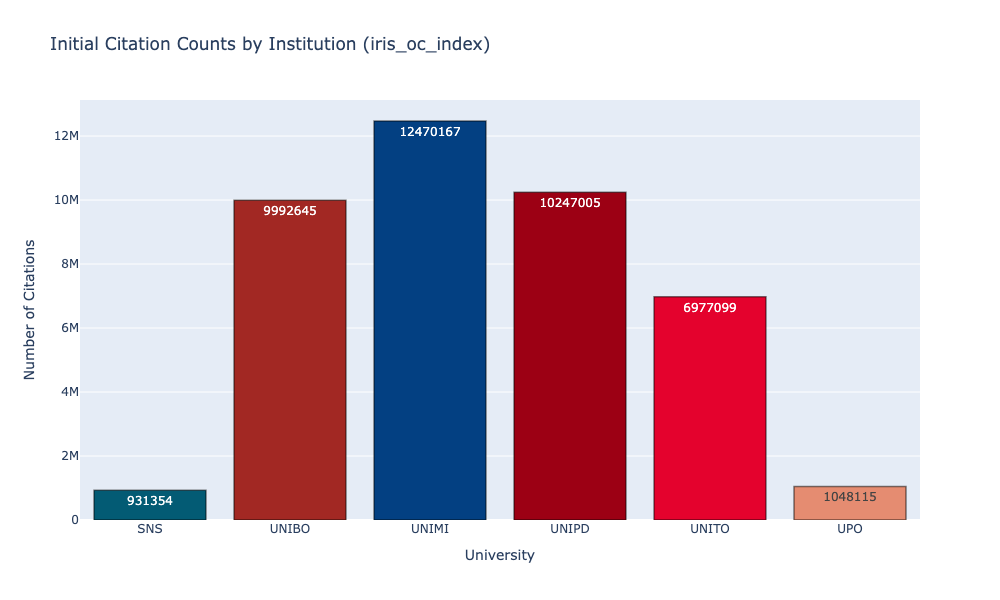
\includegraphics[width=0.75\linewidth]{img/fig1.png}
\caption{\textbf{Initial Citation Counts by Institution (\texttt{iris\_oc\_index}).}\\[1em]
Bar chart showing the total number of citations retrieved from the \texttt{iris\_oc\_index} dataset for each of the six Italian universities under study: SNS (931,354), UNIBO (9,992,645), UNIMI (12,470,167), UNIPD (10,247,005), UNITO (6,977,099), and UPO (1,048,115). UNIMI yields the highest citation volume, while SNS and UPO contribute substantially fewer records, reflecting differences in institutional size and research output.}
\label{fig1}
\end{figure}

\begin{center}
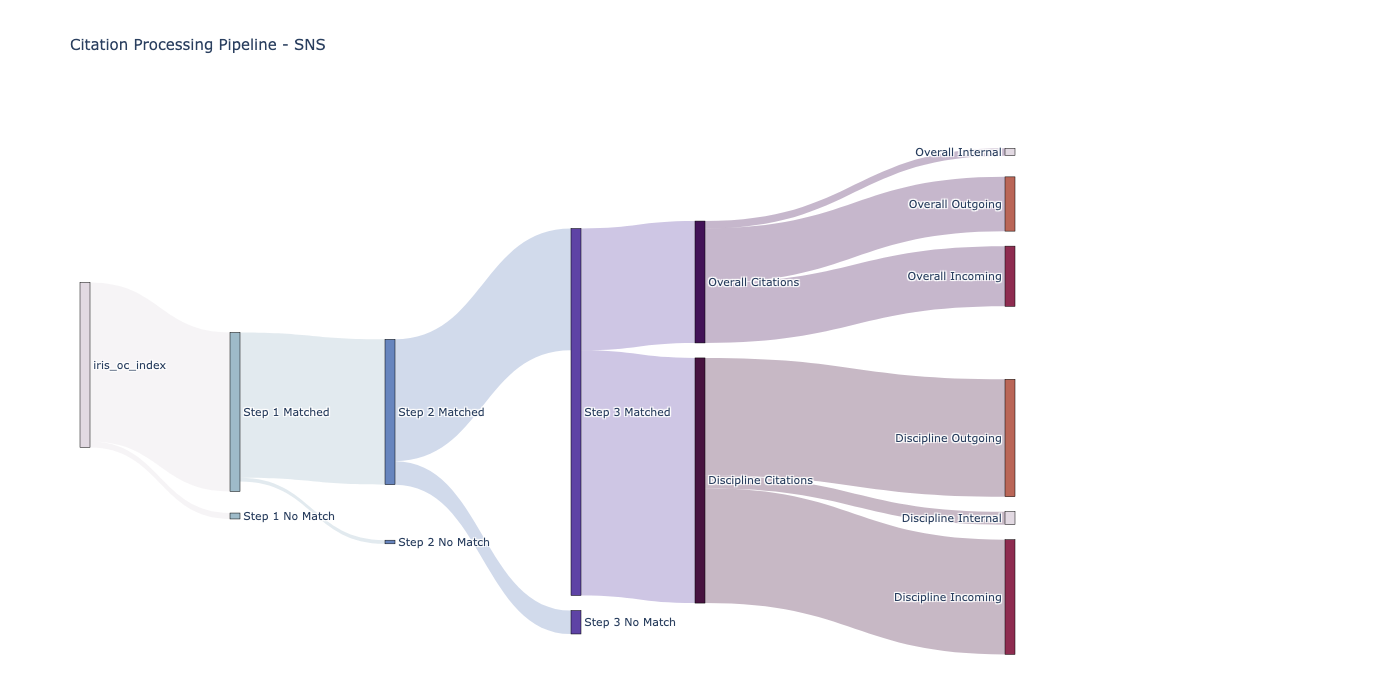
\includegraphics[width=\linewidth]{img/fig2.png}
\captionof{figure}{\textbf{Citation Processing Pipeline for SNS.}\\[1em]
Sankey diagram illustrating the record flow through the three-step data processing pipeline for the Scuola Normale Superiore (SNS). Starting from the raw \texttt{iris\_oc\_index} dataset (left), records are successively filtered at each processing stage: Step 1 (venue retrieval from OpenCitations Meta), Step 2 (ISSN-based journal classification via DOAJ and SCImago), and Step 3 (LOC alignment and standardisation). At each step, unmatched records are diverted as a separate outflow. Successfully resolved records are ultimately distributed into two output streams: Overall Citations (disaggregated by flow type into Incoming, Outgoing, and Internal) and Discipline Citations (disaggregated by the same flow types following LOC classification). Flow widths are proportional to record counts.}
\label{fig2}

\vspace{5em}

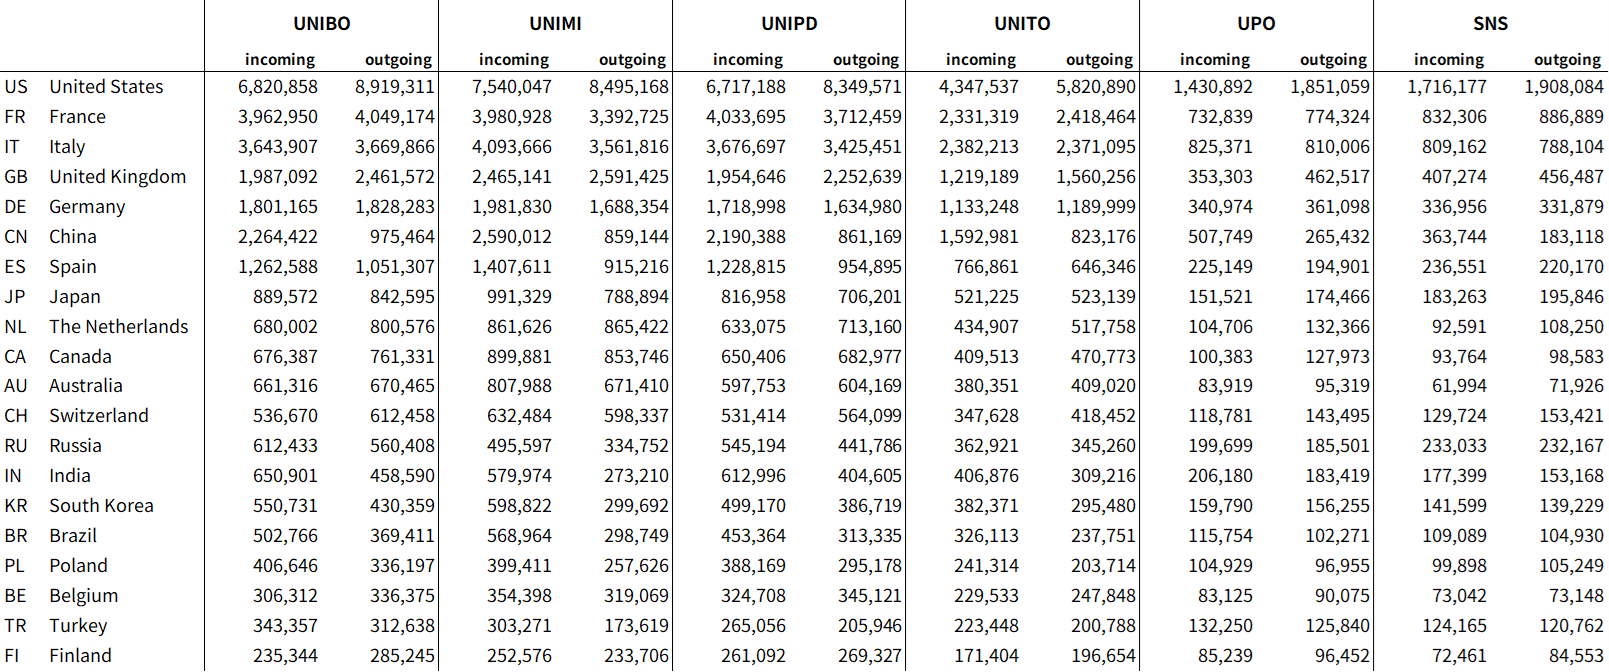
\includegraphics[width=0.75\linewidth]{img/table1.png}
\captionof{table}{\textbf{Top-20 cited and citing countries.}\\[1em]
The table lists the top-20 countries that either cite or are cited by each Italian institution. It includes the total number of citations.}
\label{tab1}
\vspace{0.5em}
\end{center}

\begin{figure}[H]
\centering
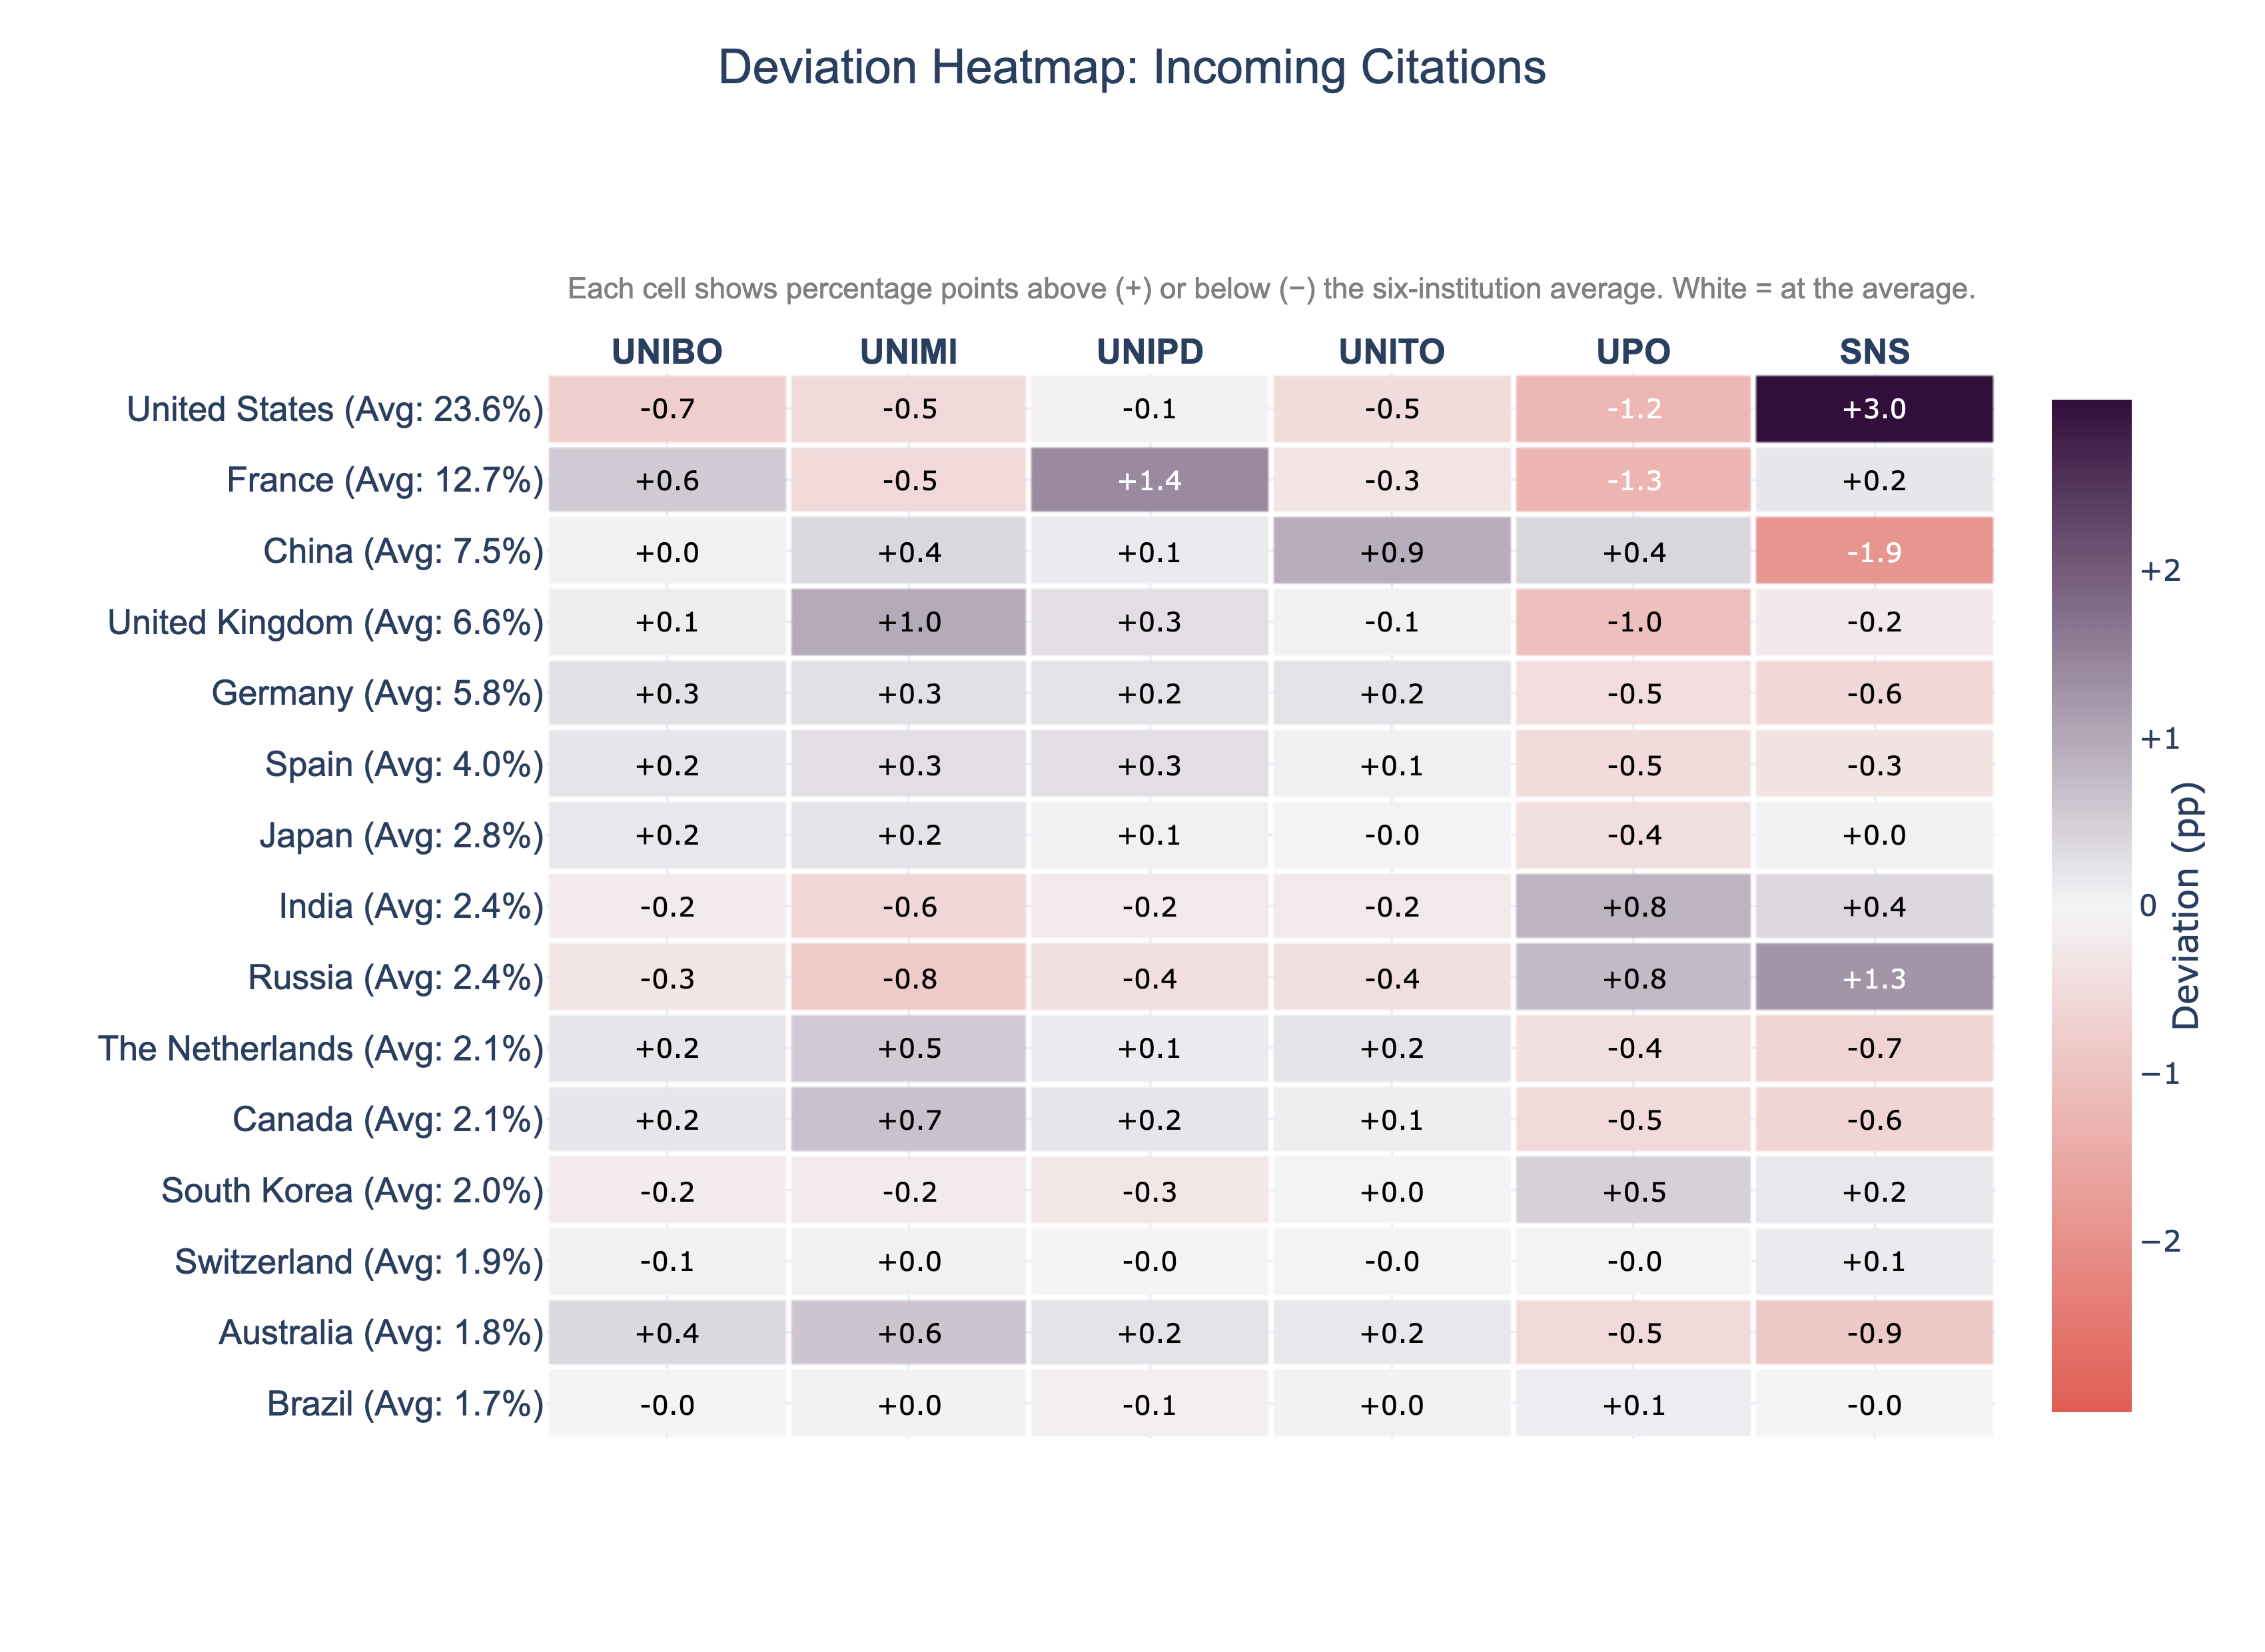
\includegraphics[width=0.75\linewidth,height=0.4\textheight,keepaspectratio]{img/fig3.png}

\vspace{1.5em}

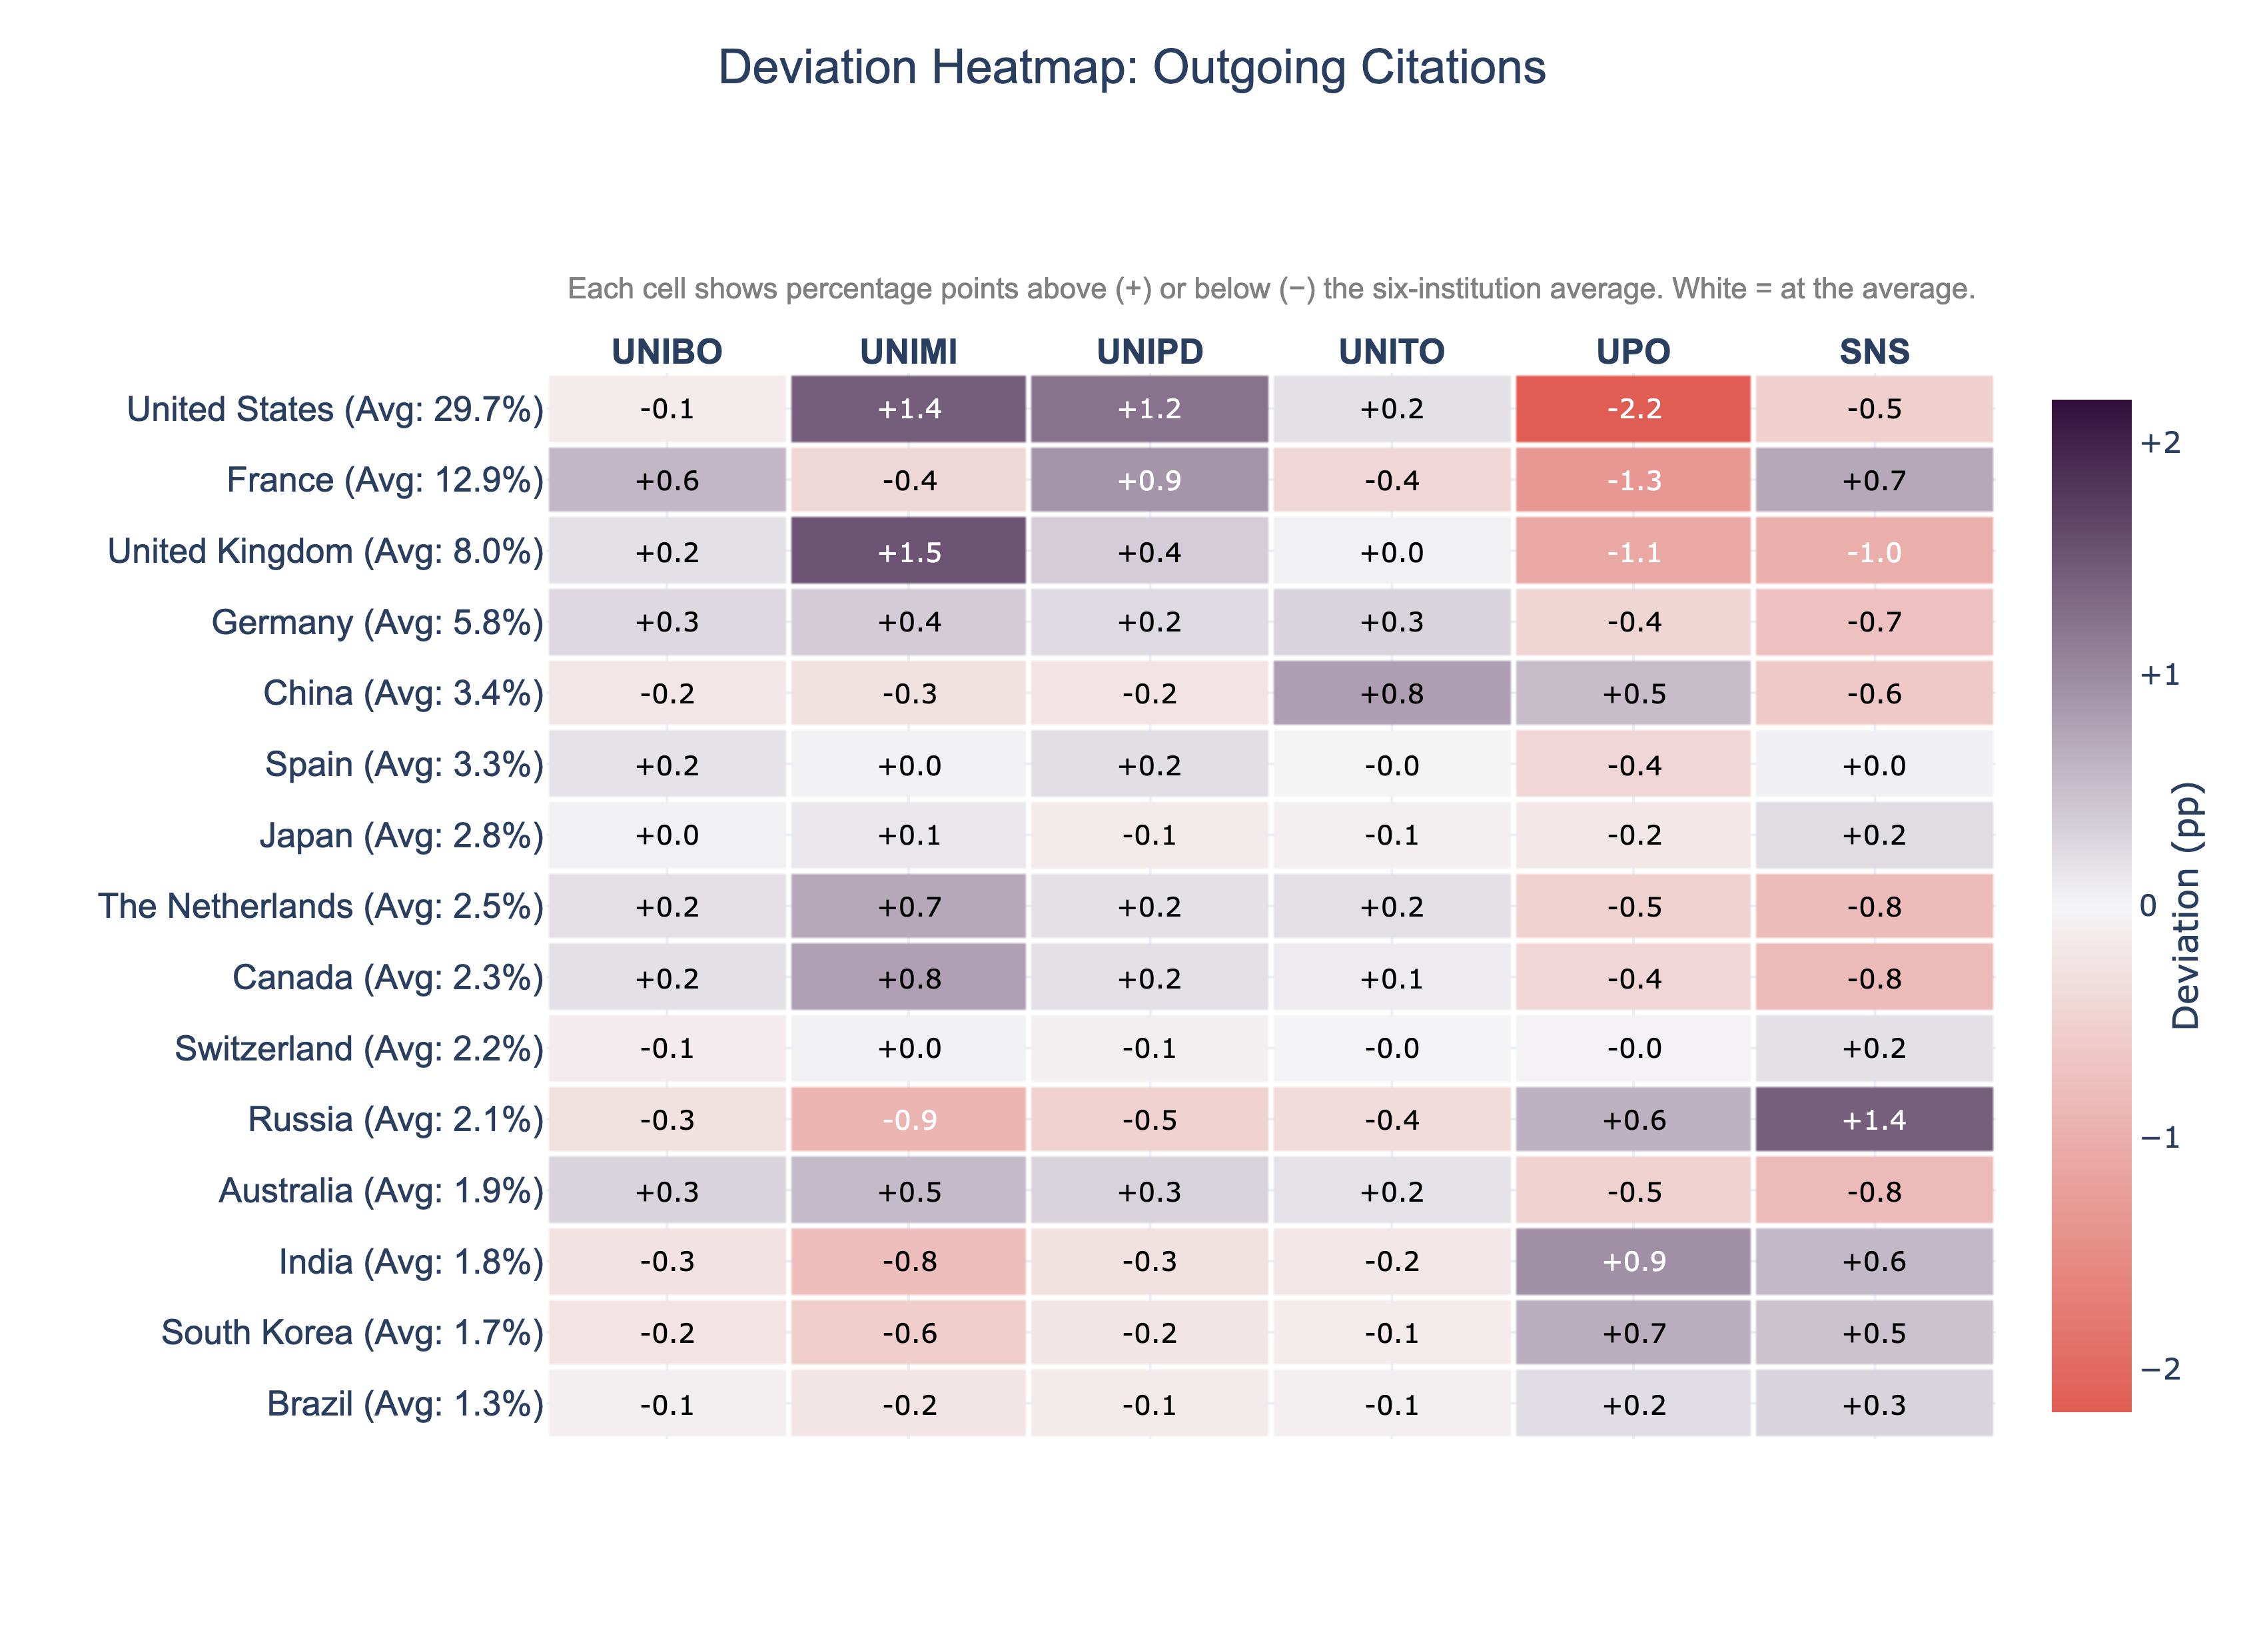
\includegraphics[width=0.75\linewidth,height=0.4\textheight,keepaspectratio]{img/fig4.png}
\caption*{\textbf{Figures 3 and 4. Diverging Heatmap for incoming and outgoing citations.}\\[1em]
Dark purple cells indicate institutions whose citation volumes deviate positively from the average pattern calculated for their respective country. Red cells indicate institutions whose citation volumes deviate negatively from the corresponding national average pattern. White cells represent the baseline, indicating that an institution’s citation flow closely matches the overall citation pattern.}
\label{fig3_4}
\end{figure}

\begin{figure}[H]
\centering
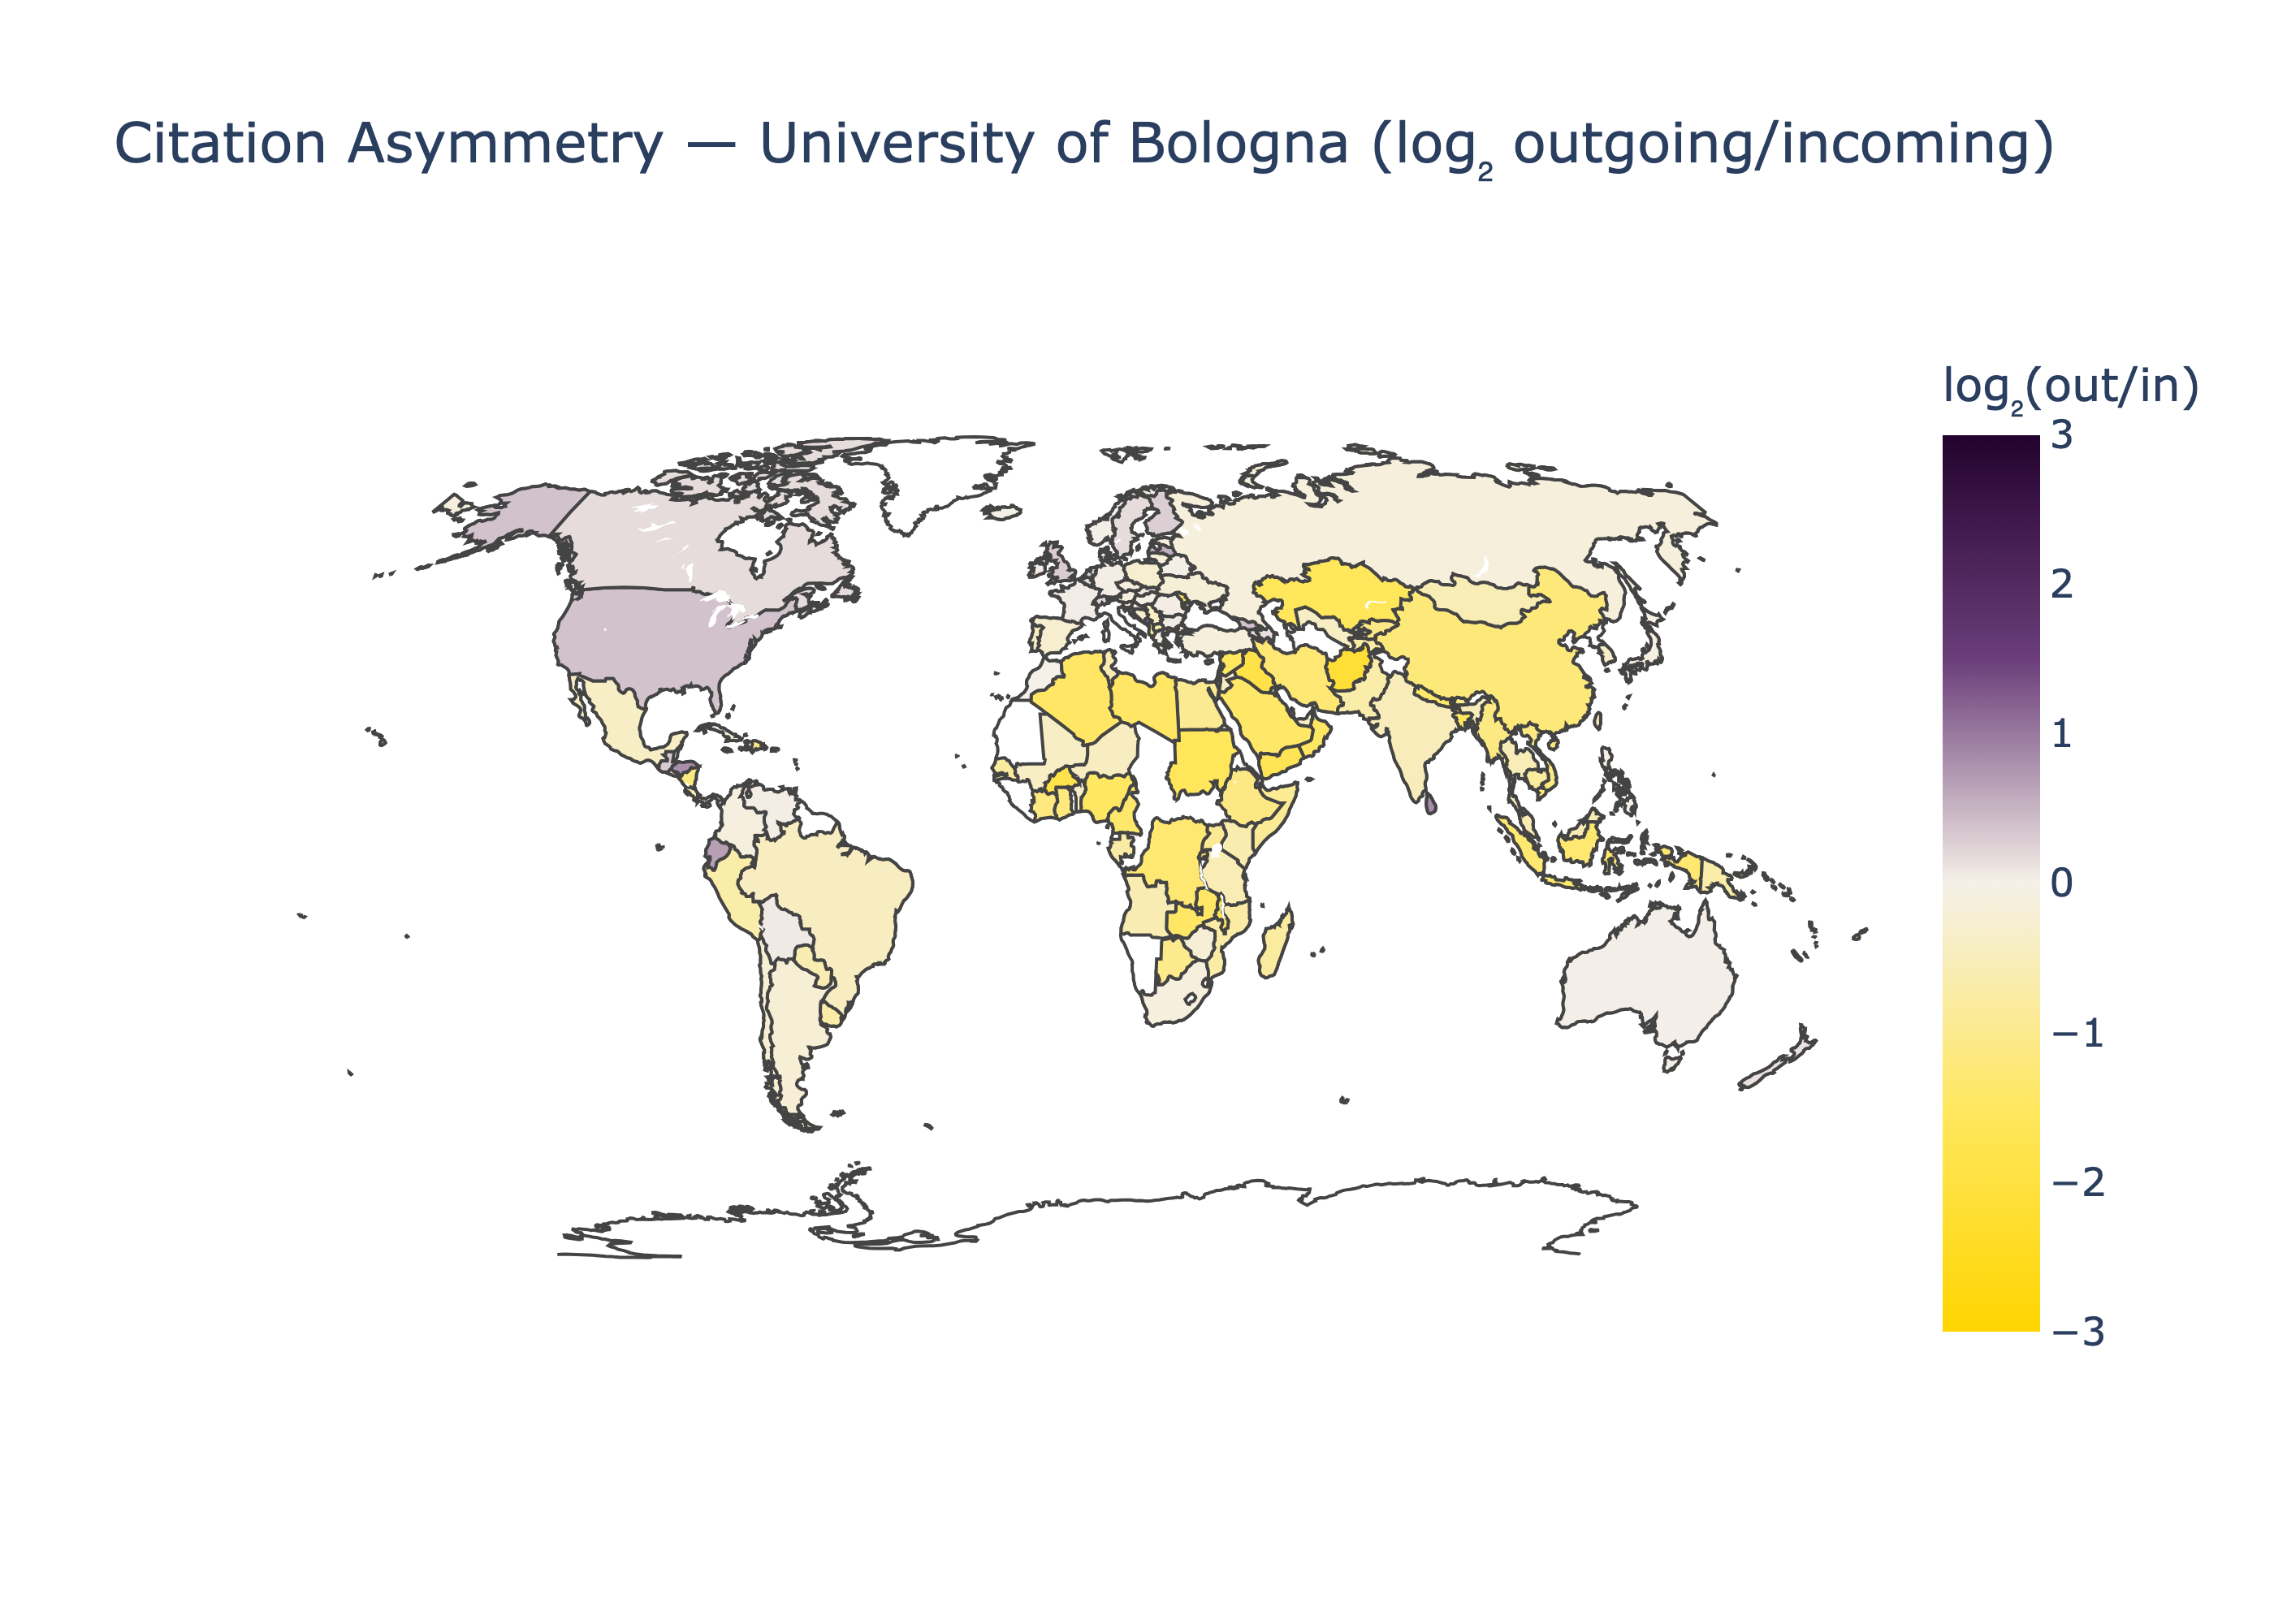
\includegraphics[width=0.75\linewidth,height=0.4\textheight,keepaspectratio]{img/fig5.png}

\vspace{1.5em}

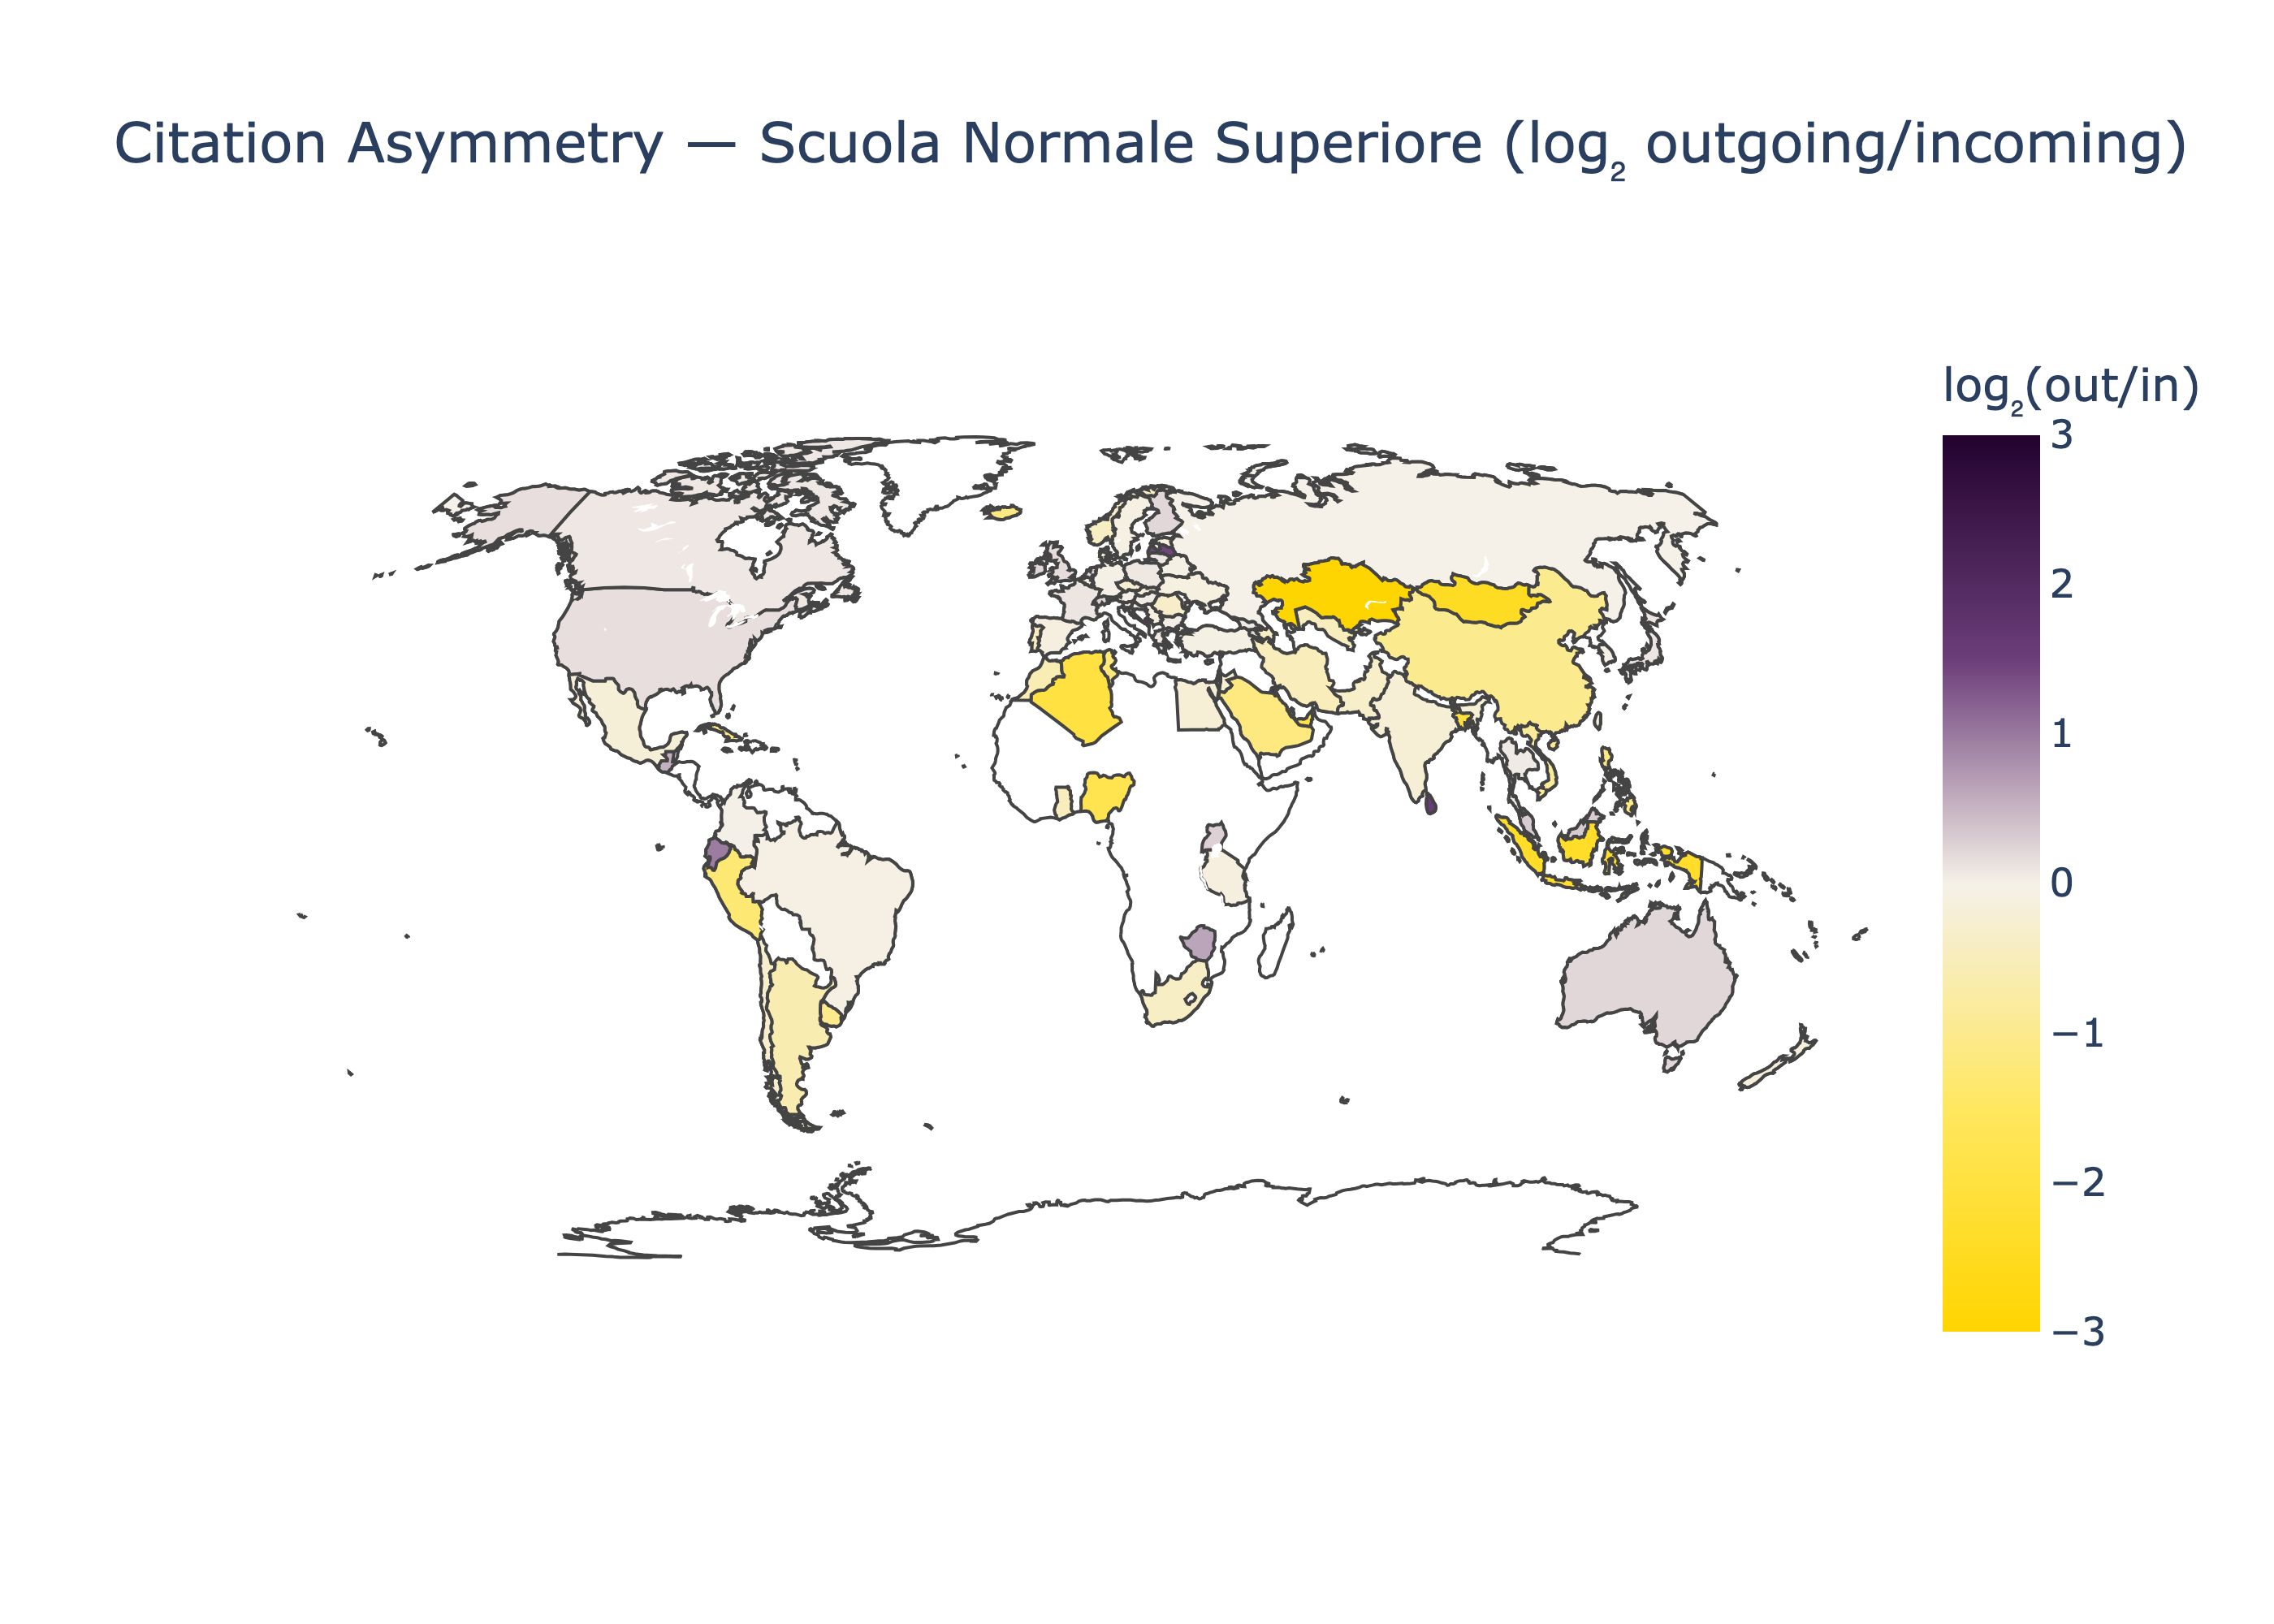
\includegraphics[width=0.75\linewidth,height=0.4\textheight,keepaspectratio]{img/fig6.png}
\caption*{\textbf{Figures 5 and 6. Asymmetry map for small institution (SNS) and large institution (UNIBO).}\\[1em]
Purple indicates an outgoing citation bias, meaning that a specific country is a knowledge provider; white shows reciprocal balance; gold-yellow signals an incoming bias, yellow countries act as knowledge consumer.}
\label{fig5_6}
\end{figure}

\begin{figure}[H]
\setcounter{figure}{6}
\centering
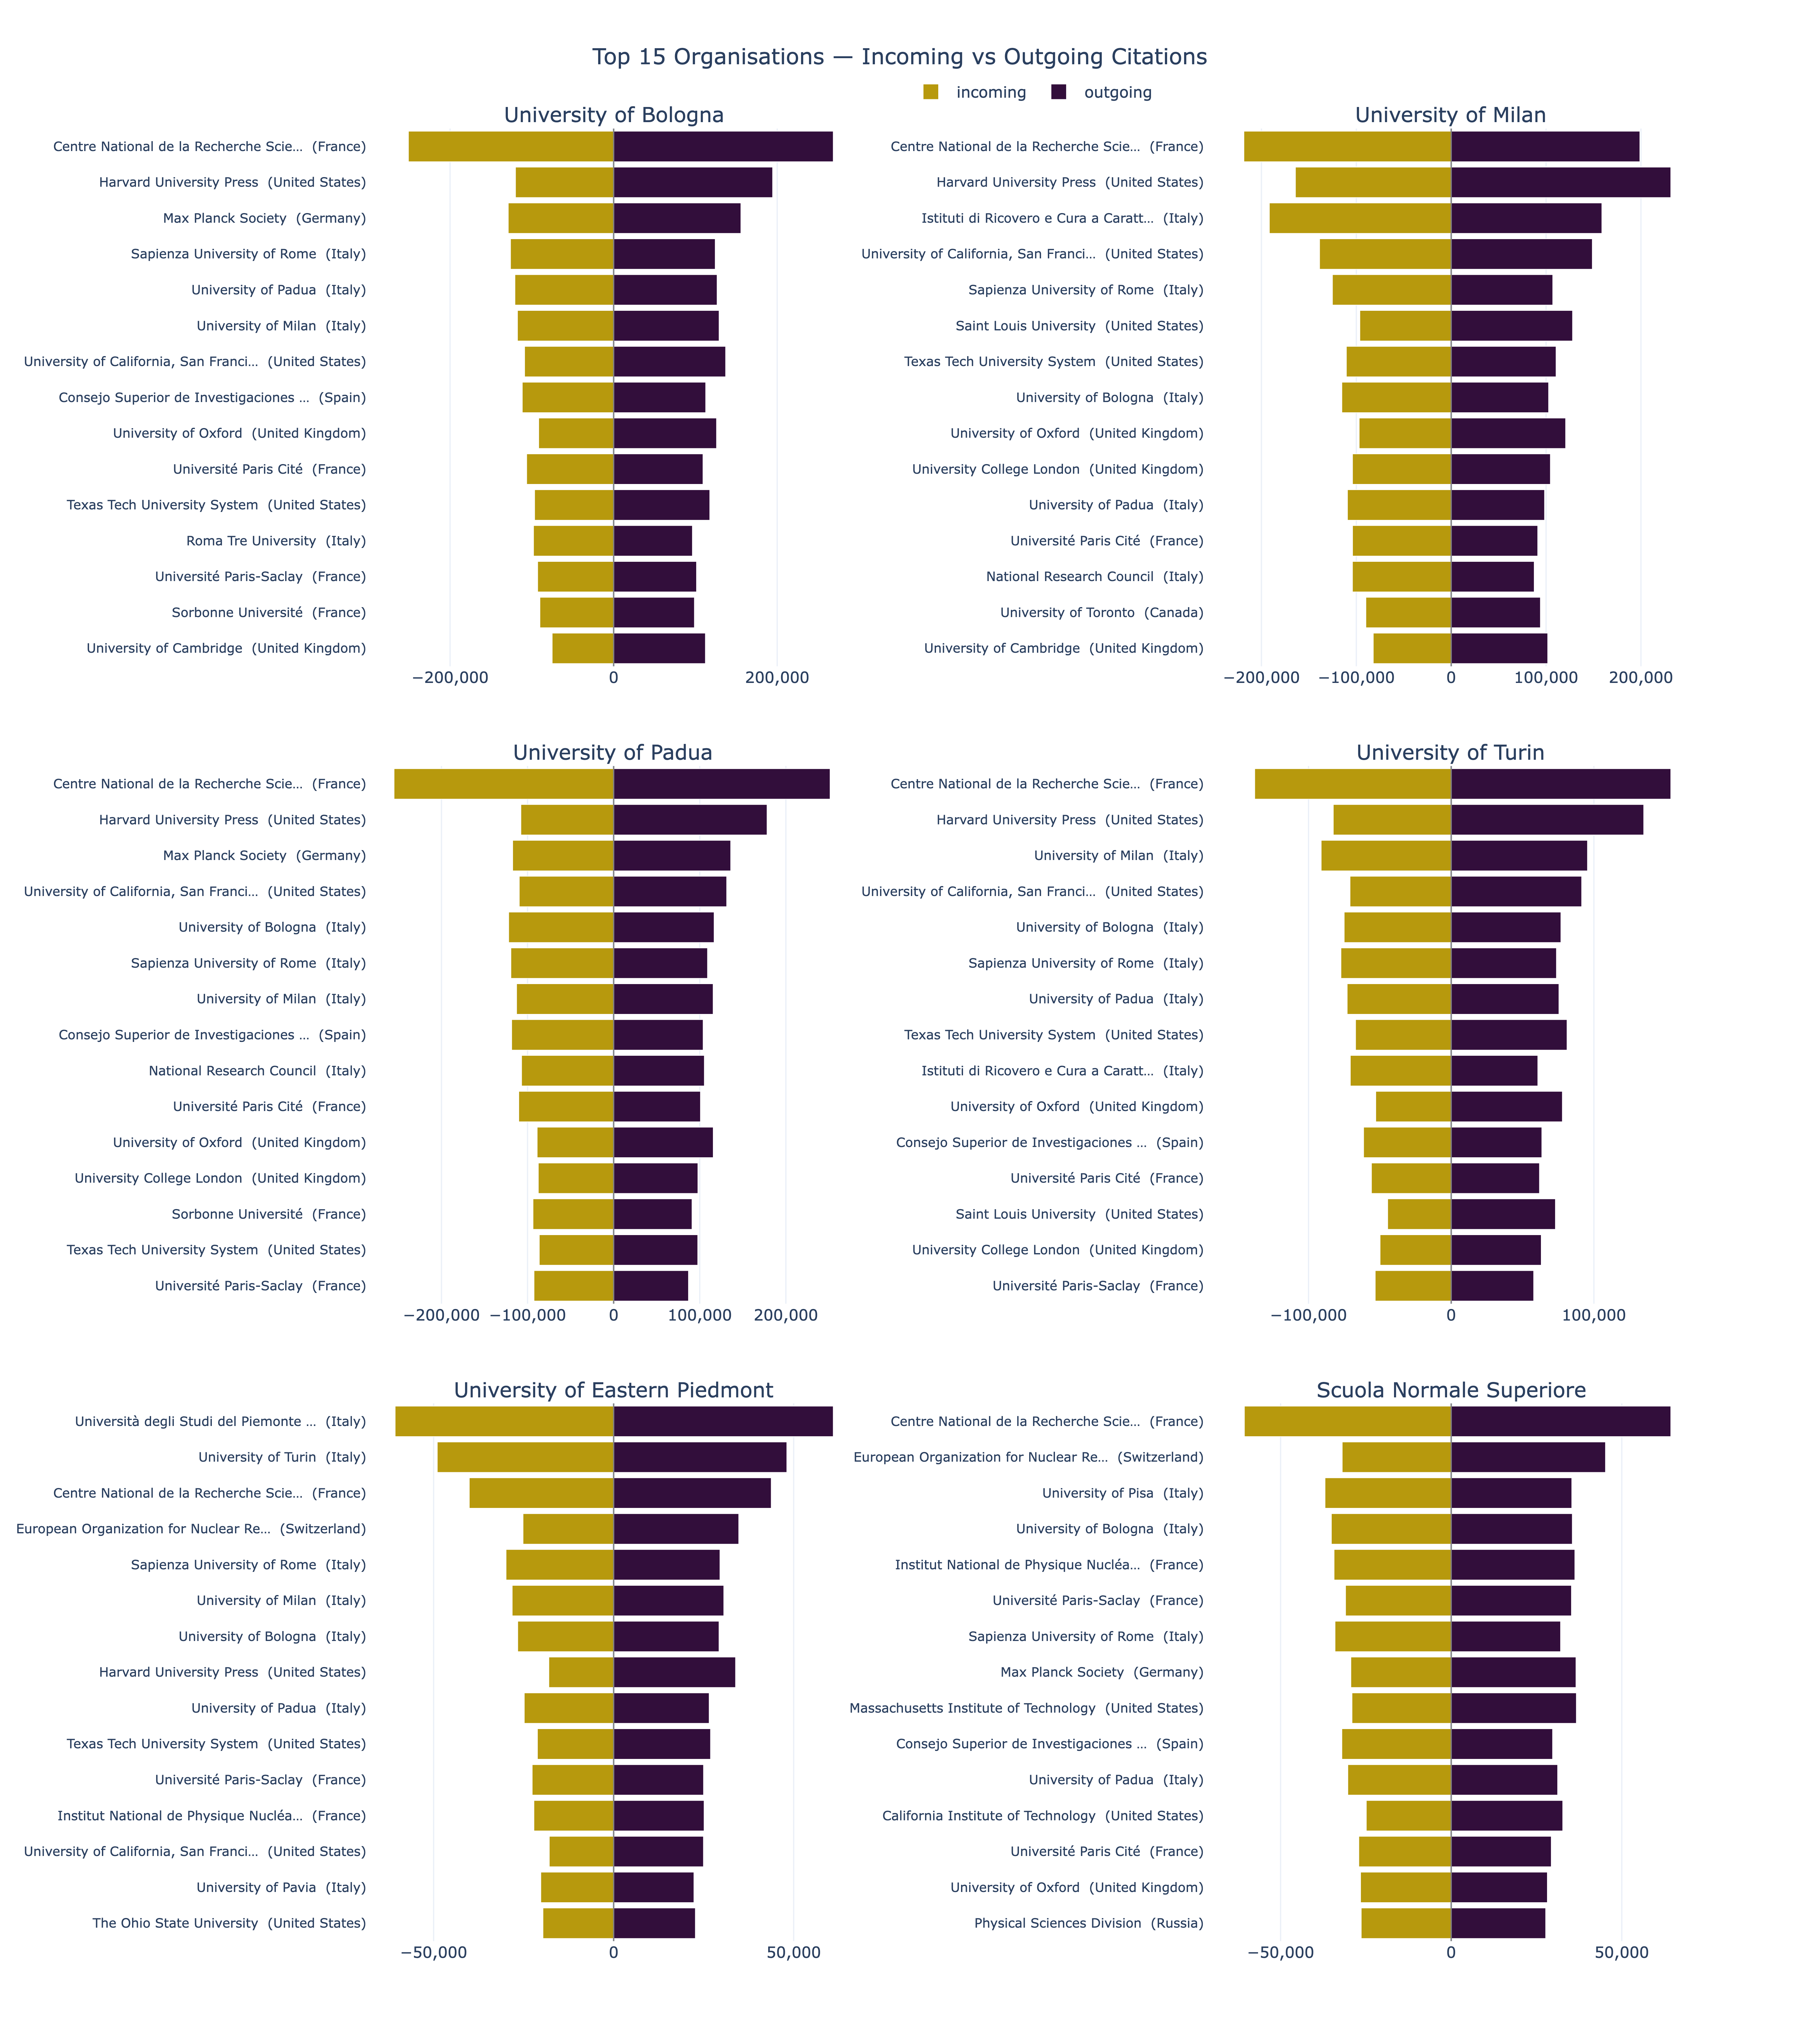
\includegraphics[width=0.75\linewidth,height=0.85\textheight,keepaspectratio]{img/fig7.png}
\caption{\textbf{Butterfly Charts.}\\[1em]
Each chart shows the top-15 partner organizations ranked by total citation volume, incoming and outgoing combined. Bars extending left indicate the organizations that cite the focal institution (incoming); bars extending right indicate organizations cited by the focal institution (outgoing).}
\label{fig7}
\end{figure}

\newpage
\begin{center}
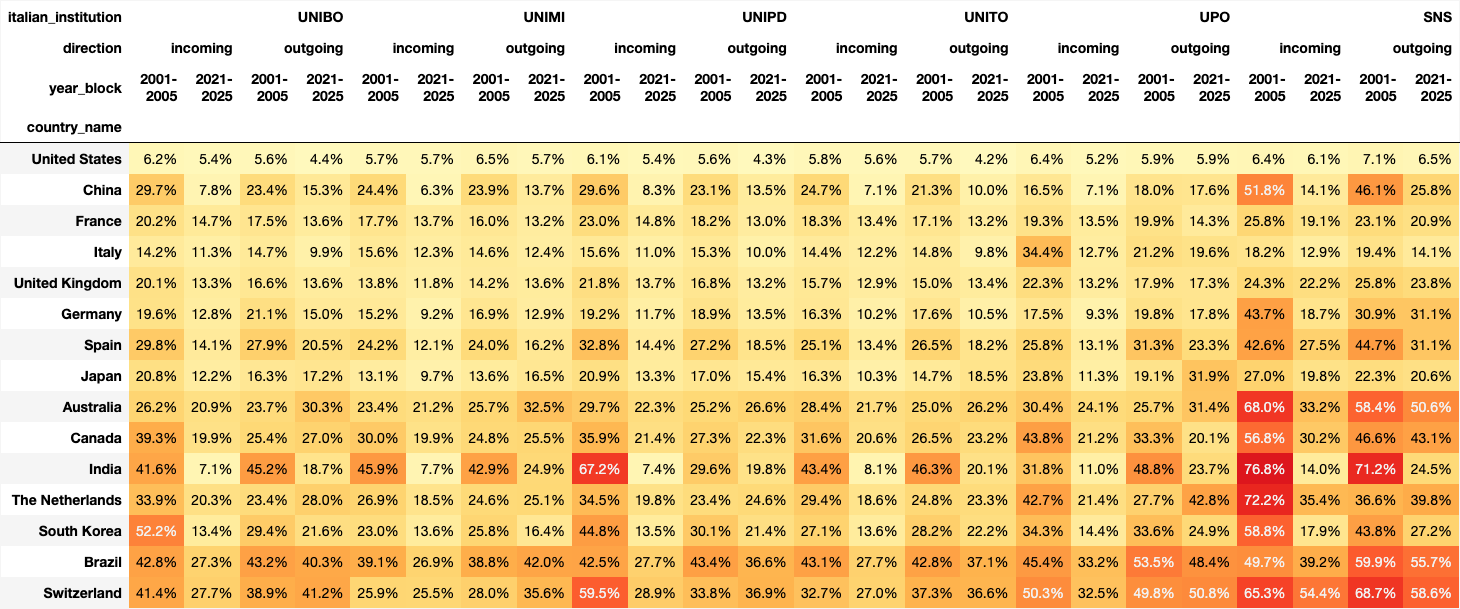
\includegraphics[width=0.75\linewidth,height=0.85\textheight,keepaspectratio]{img/table2.png}
\vspace{0.5em}
\captionof{table}{\textbf{Citation Concentration vs Volume.}\\[1em]
The table reveals the concentration metrics for each country related to the total volume of citations. It answers the question whether an institution relies on a large network of organizations or a smaller one concentrated in one or two organizations. Red indicates a high concentration, meaning citations are concentrated into a small system of organizations; yellow indicates a low concentration, citations in those countries are more distributed. The table contains temporal data, exploring how the structure evolves over time.}
\label{tab2}
\end{center}

\begin{figure}[H]
\centering
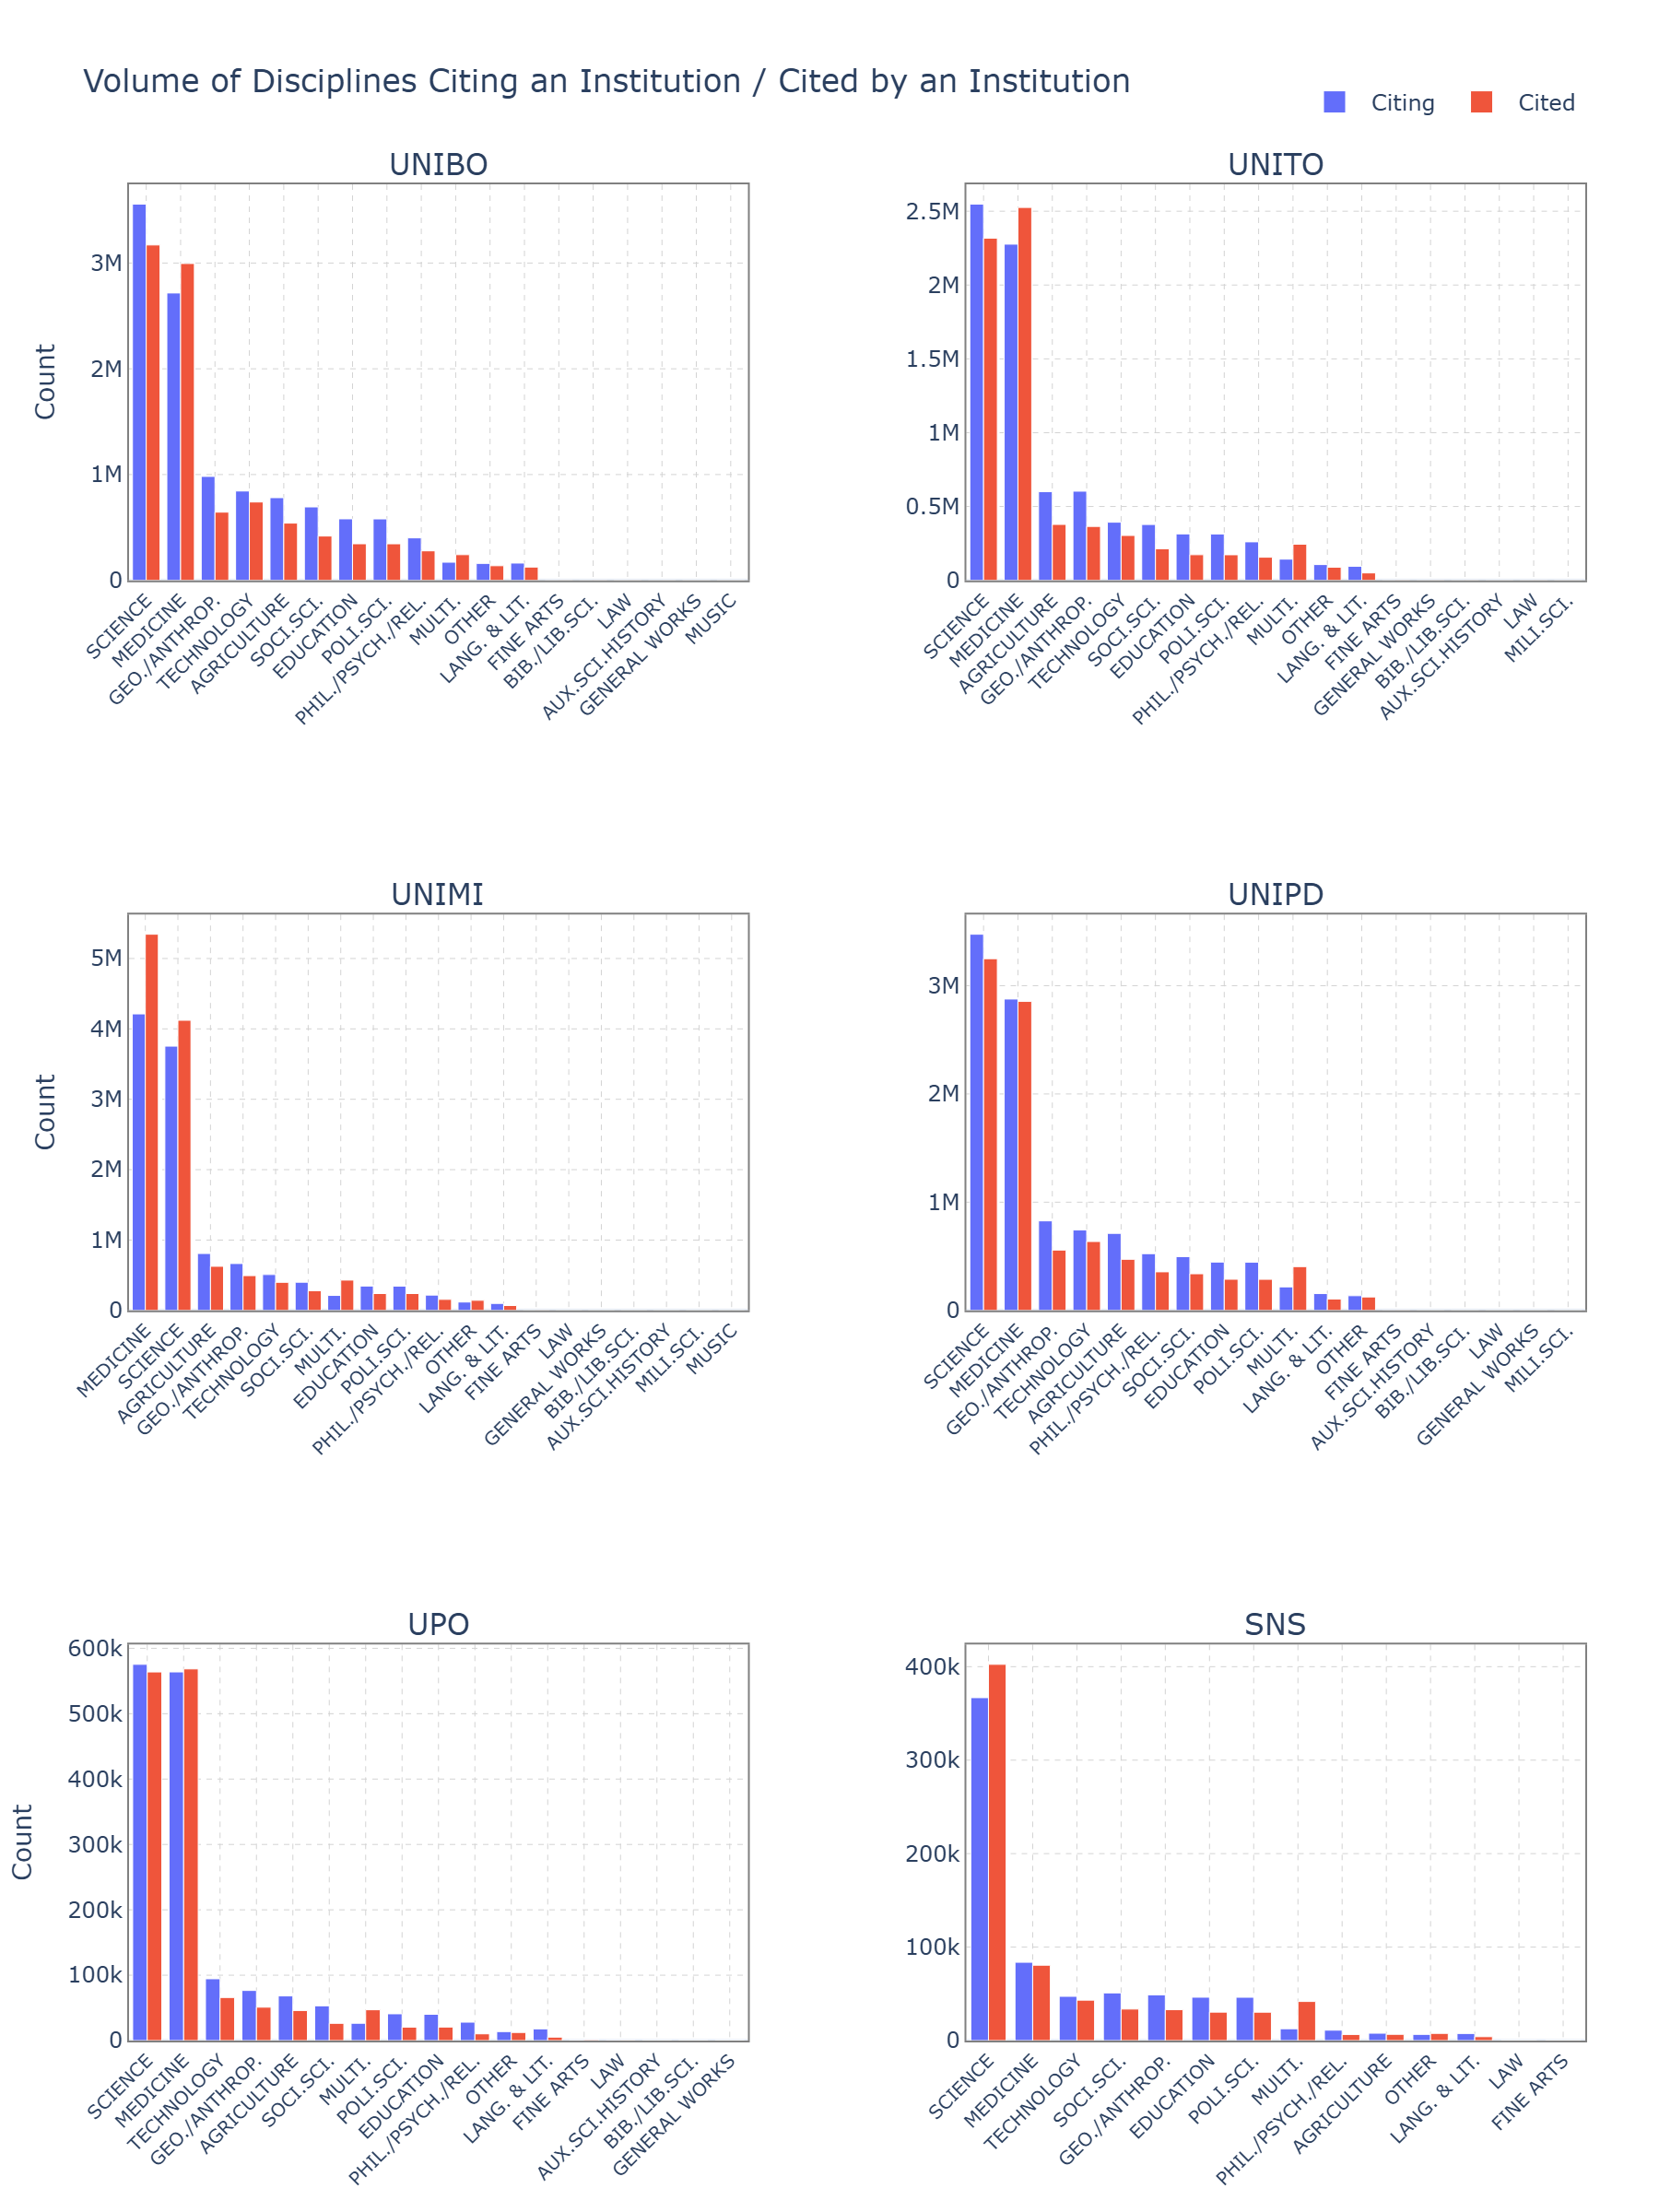
\includegraphics[width=0.75\linewidth,height=0.85\textheight,keepaspectratio]{img/fig8.png}
\caption{\textbf{Volume of Disciplines Citing an Institution / Cited by an Institution across Six Italian Universities.}\\[1em]
Grouped bar charts showing the total citation volume per discipline for each of the six institutions (UNIBO, UNITO, UNIMI, UNIPD, UPO, and SNS). Blue bars represent the number of citation actions in which a given discipline cites the institution's publications (Citing), while red bars represent the number of citation actions in which the institution's publications are cited by a given discipline (Cited). Disciplines are labelled using abbreviated forms of the Library of Congress Classification main classes and are ordered by total citation volume in descending order. Note that y-axis scales differ across panels to accommodate the varying citation volumes of individual institutions.}
\label{fig8}
\end{figure}

\begin{figure}[H]
\centering
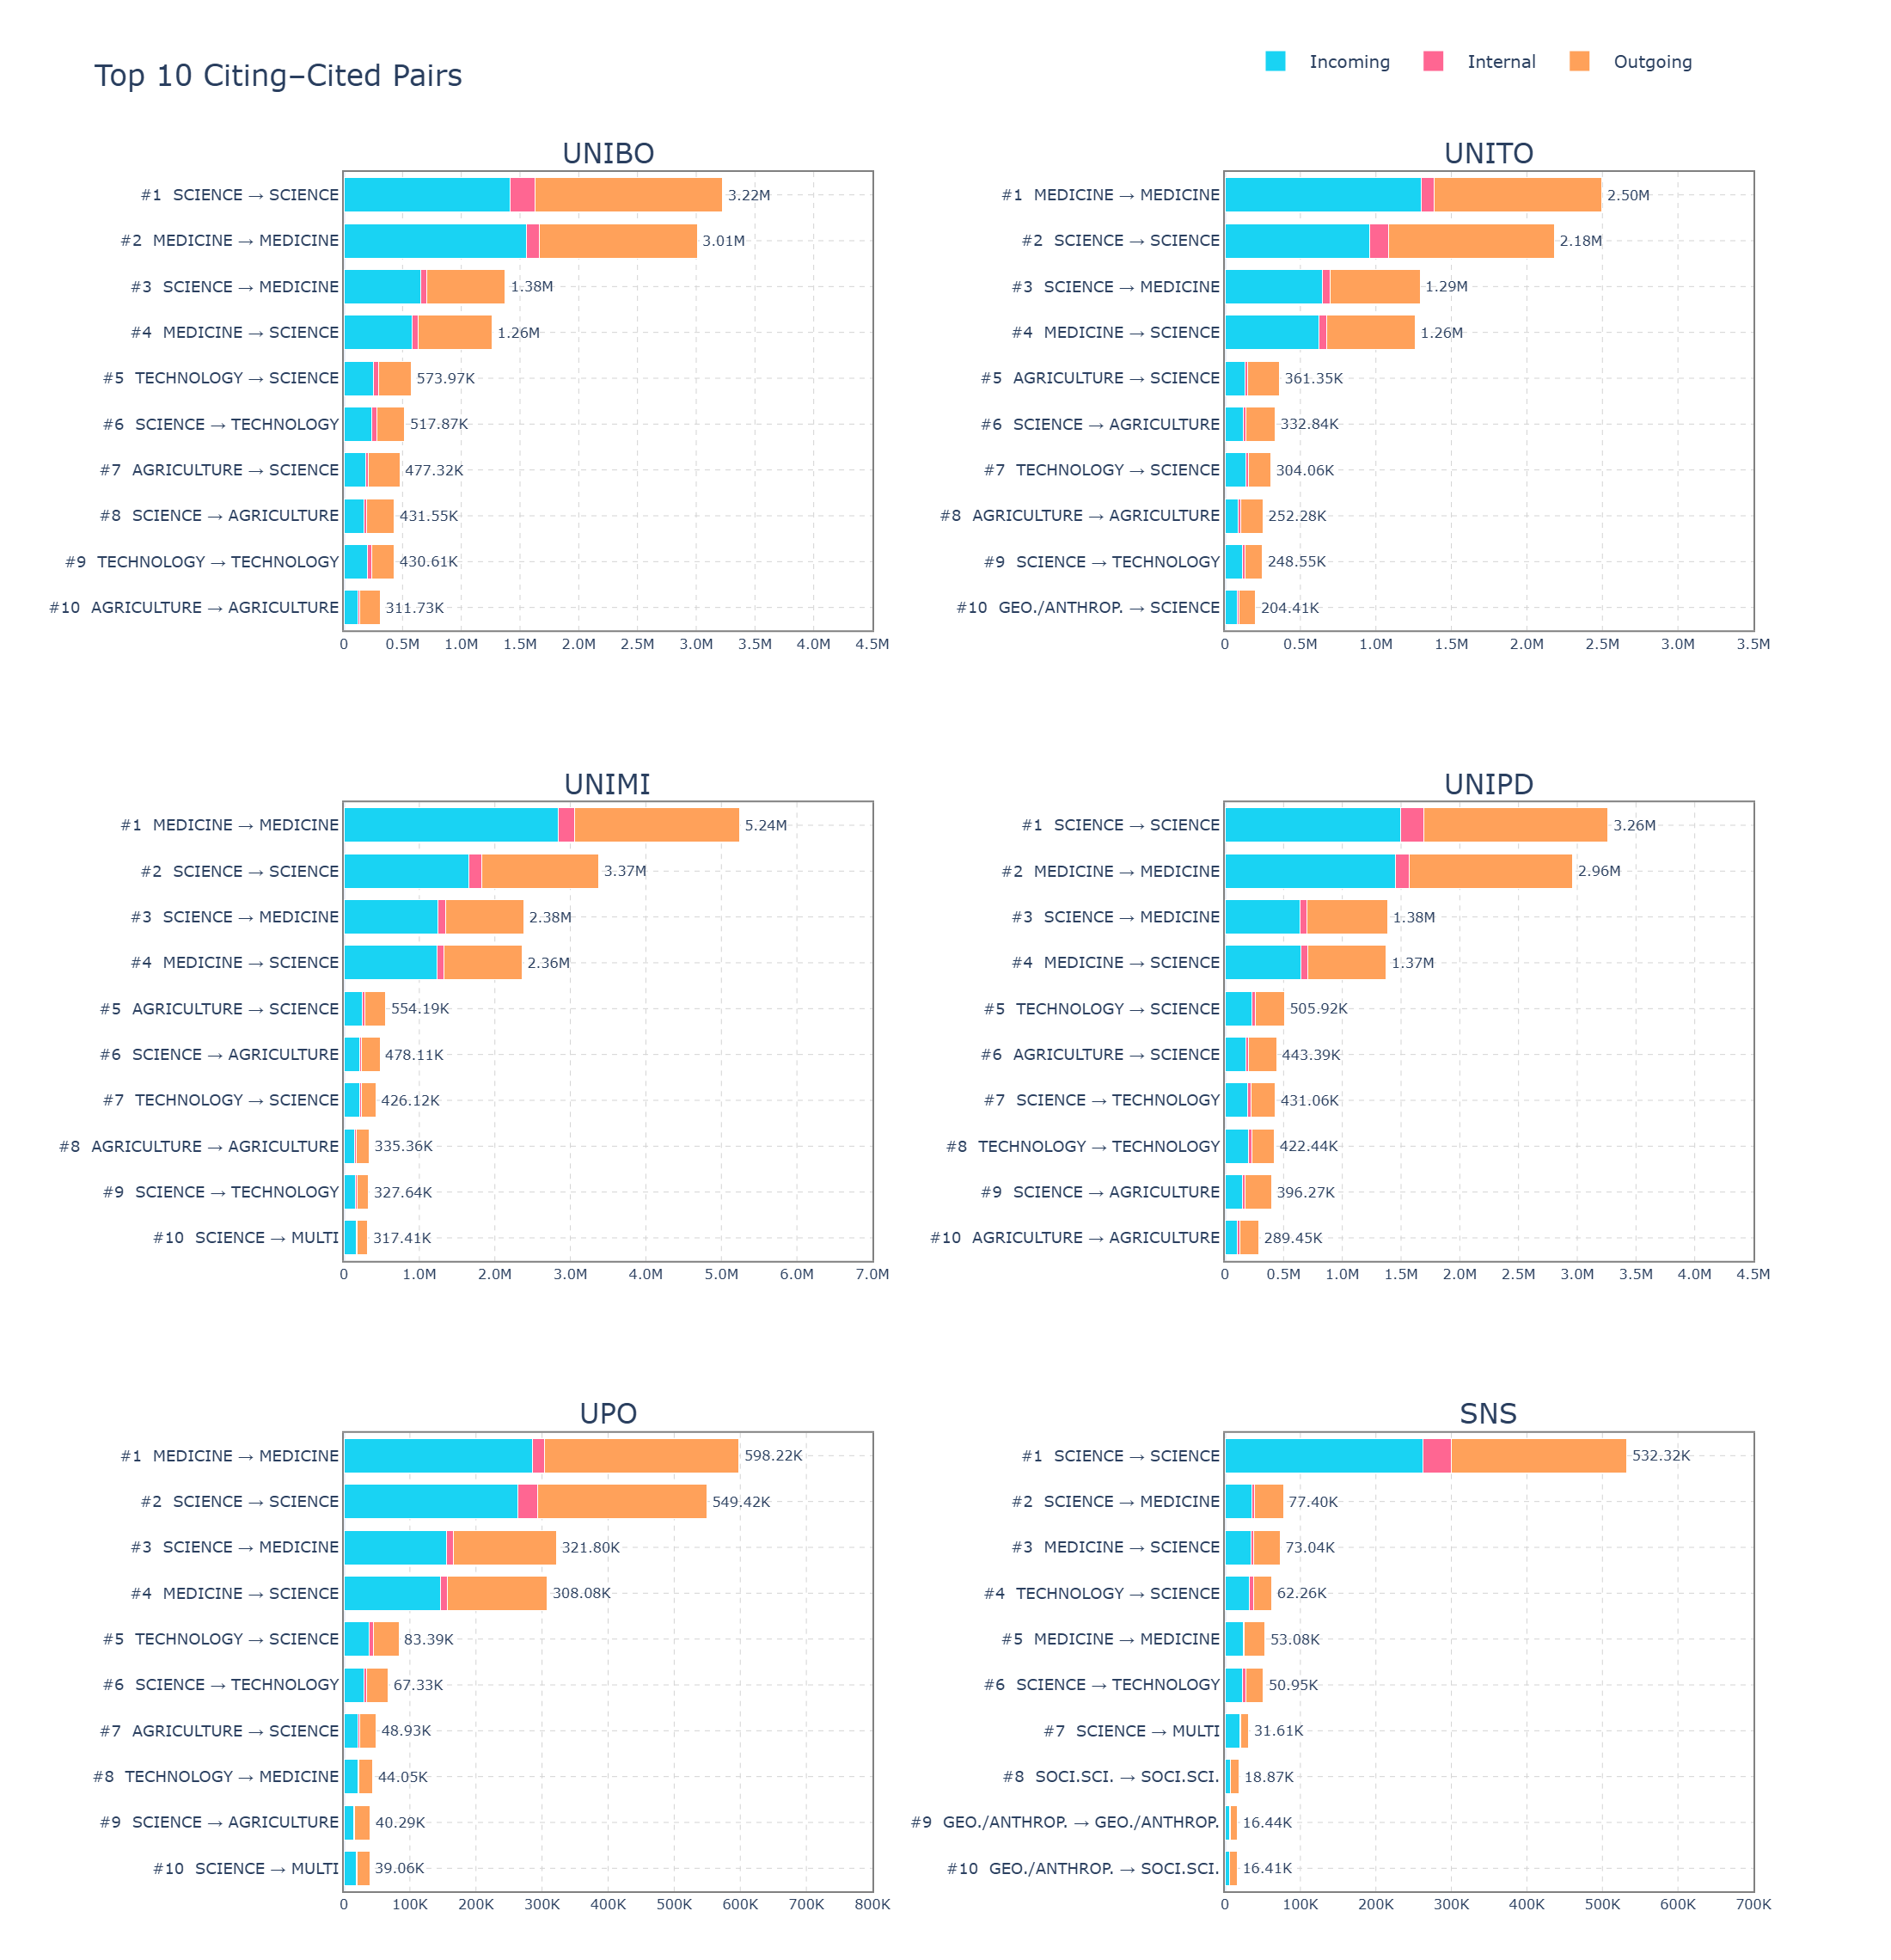
\includegraphics[width=0.75\linewidth,height=0.85\textheight,keepaspectratio]{img/fig9.png}
\caption{\textbf{Top 10 Citing–Cited Discipline Pairs by Institution.}\\[1em]
Horizontal bar charts showing the ten most frequent discipline-to-discipline citation pairs for each of the six institutions (UNIBO, UNITO, UNIMI, UNIPD, UPO, and SNS). Each bar represents the total volume of citation actions between a source discipline (citing) and a target discipline (cited), disaggregated by citation flow type: Incoming (cyan), Internal (pink), and Outgoing (orange). Pairs are ranked in descending order of total citation volume. Note that x-axis scales differ across panels to accommodate the varying citation volumes of individual institutions.}
\label{fig9}
\end{figure}

\begin{figure}[H]
\centering
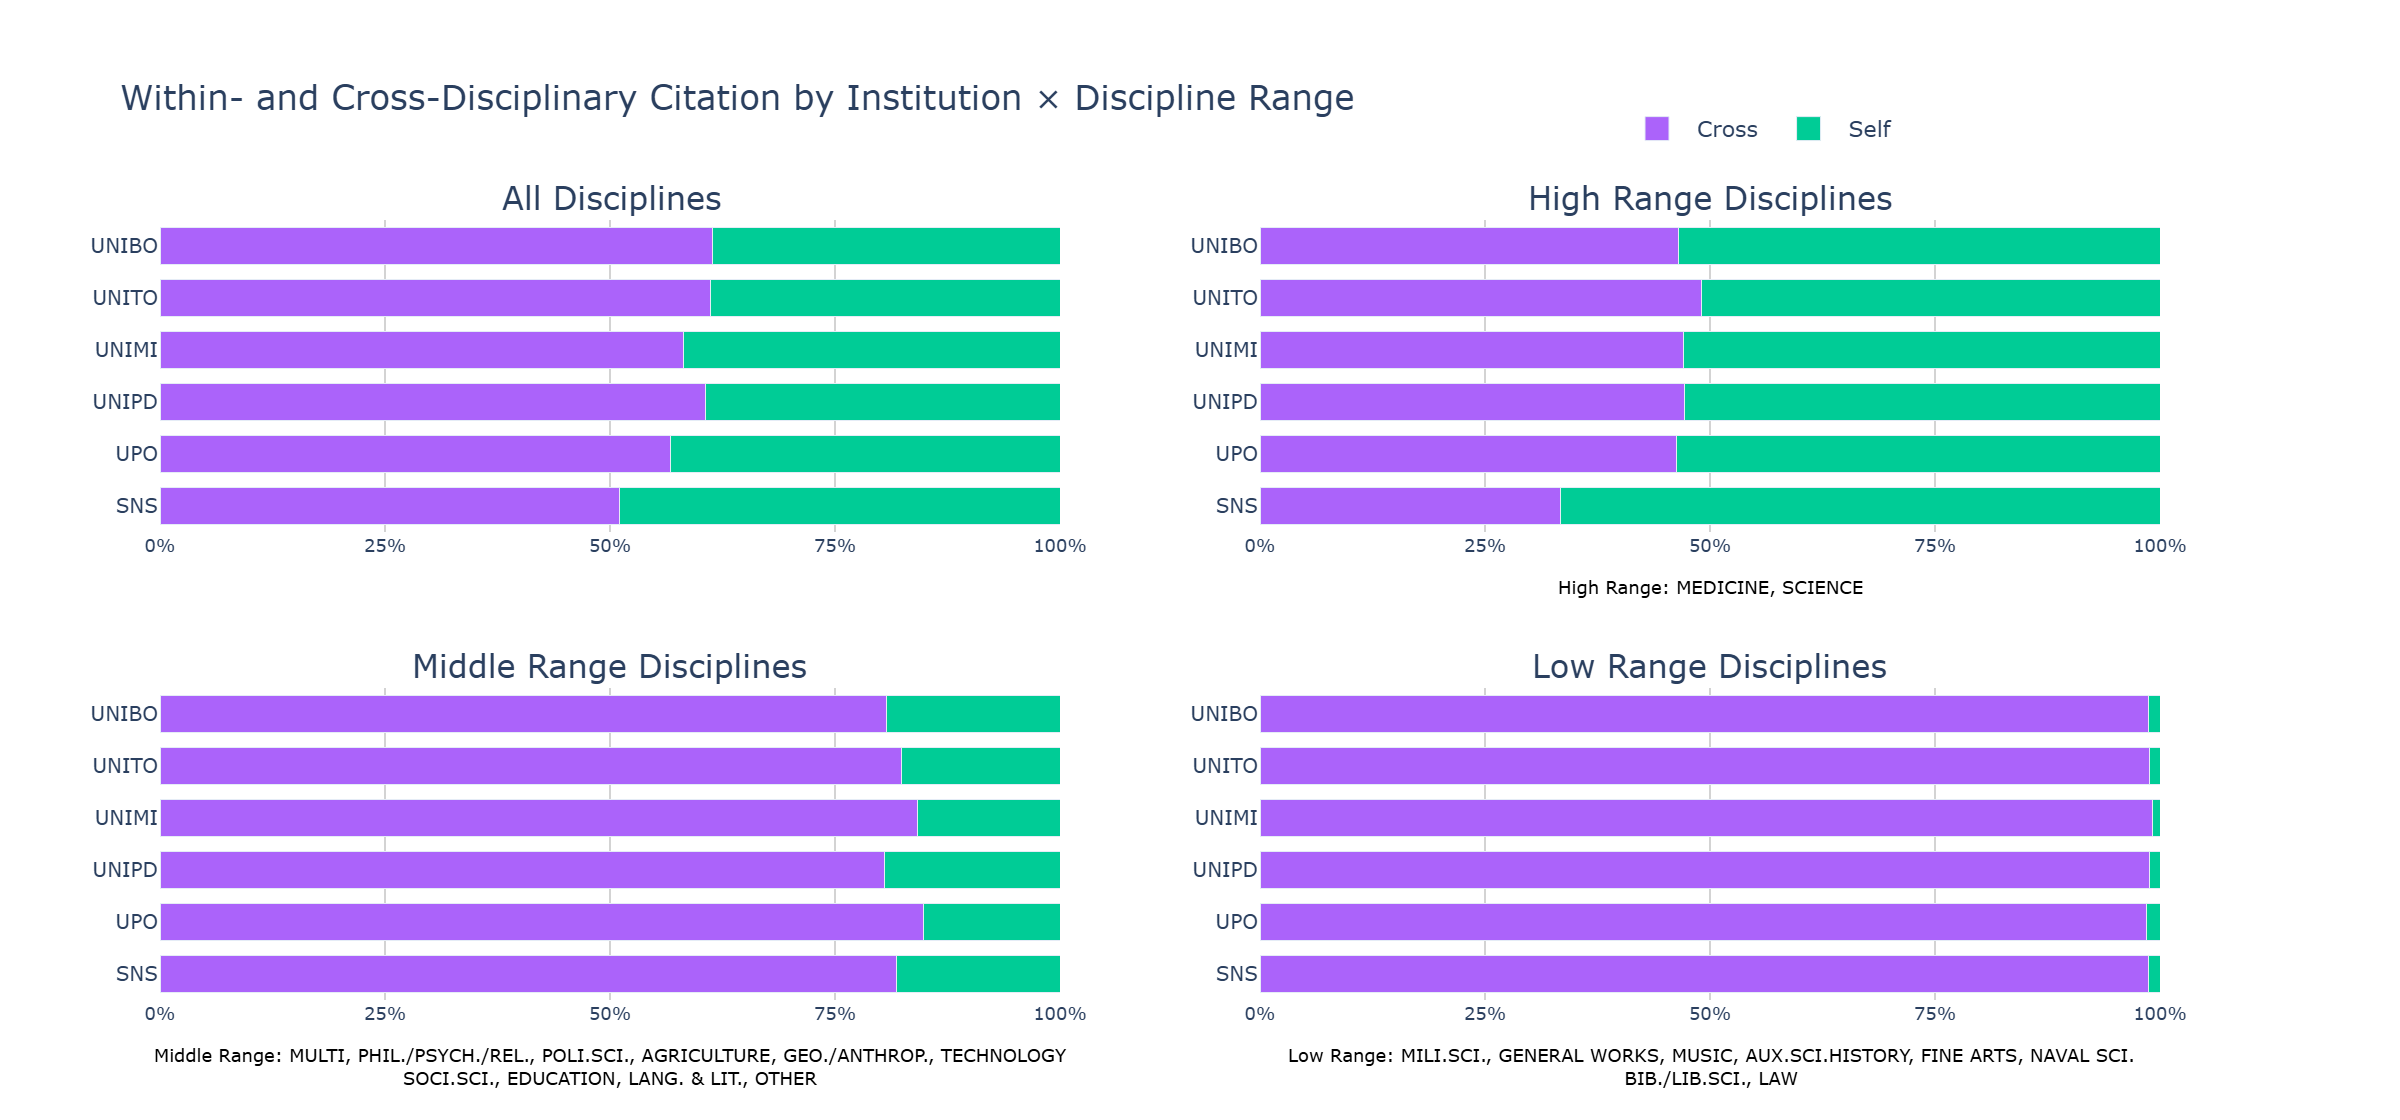
\includegraphics[width=0.75\linewidth,height=0.85\textheight,keepaspectratio]{img/fig10.png}
\caption{\textbf{Within- and Cross-Disciplinary Citation Proportions by Institution and Discipline Range.}\\[1em]
100\% stacked bar charts showing the proportion of within-discipline (Self, green) and cross-disciplinary (Cross, purple) citation actions for each institution, disaggregated across four discipline range groups: All Disciplines, High Range (Medicine and Science), Middle Range (including Multidisciplinary, Philosophy/Psychology/Religion, Political Science, Agriculture, Geography/Anthropology, Technology, Social Sciences, Education, Language and Literature, and Others), and Low Range (including Military Science, General Works, Music, Auxiliary Sciences of History, Fine Arts, Naval Science, Bibliography/Library Science, and Law). Each bar sums to 100\%, representing the relative share of self and cross citation within each group.}
\label{fig10}
\end{figure}

\vspace{4em}

\begin{center}
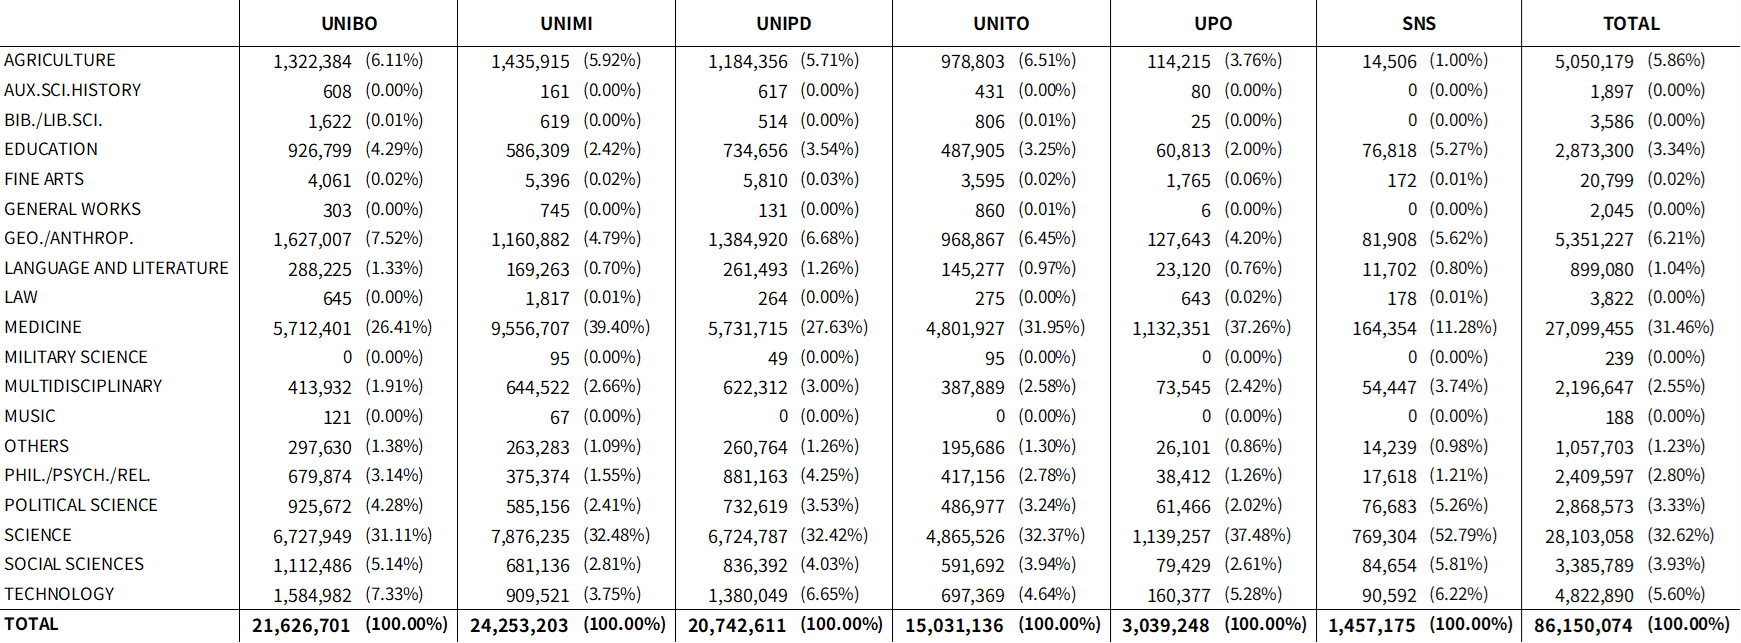
\includegraphics[width=0.75\linewidth,height=0.85\textheight,keepaspectratio]{img/table3.png}

\vspace{0.5em}

\captionof{table}{\textbf{Total citation records and share per discipline [1B - Results].}\\[1em]
Citation counts and percentage shares for each Library of Congress Classification main class across the six participating institutions (UNIBO, UNIMI, UNIPD, UNITO, UPO, and SNS), combining citing and cited activity. Percentages represent each discipline's share of the institution's total citation volume. The rightmost column reports the aggregate totals across all six institutions. Disciplines with near-zero counts (e.g., Military Science, Music, General Works) reflect limited coverage of these fields within the classification sources used in this study.}
\label{tab3}
\end{center}

\end{document}